\documentclass[a4paper,12pt]{article}
\usepackage{partiiiessay}


\title{\vspace{-40pt} Basis Reduction in Lattice Cryptography}
% \author{\vspace{-10pt}Raj Kane}
% \date{%
% May 2019
% }
% used https://www.overleaf.com/2460029rpwpbr#/6413425/

\begin{document}
\vspace{-45pt}
\begin{titlepage}
    \begin{center}
        \vspace*{5cm}%
        {\LARGE Basis Reduction in Lattice Cryptography}\\[1cm]
        {\normalsize Raj Kane}\\[0.5cm]
        {\normalsize Honors Thesis}\\[0.5cm]
        {\normalsize Mathematics Department}\\[0.5cm]
        {\normalsize Colby College}\\[0.5cm]
        {\normalsize May 2019}\\[0.5cm]
        %...
    \end{center}
    \let\newpage\relax% Avoid following page break
\end{titlepage}
\newpage
\tableofcontents
\clearpage

% ************************************************************************
% Acknowledgements
% ************************************************************************
\section{Acknowledgements}

I would like to begin by thanking Professor Nora Youngs for her advice and patience throughout this year. This paper would not have been possible without her help. 

This paper would also not have been possible without Professor David Krumm, who fed my interest in cryptography and suggested that I look into lattices.

Next, I would like to thank Professor Leo Livshits for agreeing to be a reader for this paper and providing many helpful suggestions.

I also would like to thank Professors Livshits, Krumm, Scott Taylor, Evan Randles, and Fernando Gouv$\hat{\text{e}}$a for their guidance through the world of math. I am incalculably grateful for all their instruction.

Finally, I would like to thank my friends, especially Shabab Ahmed, Brian Long, Yashaswi Mohanty, and Kyle McDonell, for their constant support and faith throughout my mathematical and collegiate journeys. 

\newpage

% ************************************************************************
% Introduction
% ************************************************************************
\section{Introduction}

Cryptography stems from the desire to secure private communications in the face of unwanted eavesdroppers. Developments in ensuring the secrecy of messages have been spurred by developments in cryptanalysis: the study of finding ways to gain unintended access to private communications by third parties. The field has grown from simple Caesar ciphers to the RSA cryptosystem and beyond. Now, cryptography is a heavily mathematical field, with new systems of cryptography (or \textit{cryptosystems}) being designed around difficult mathematical problems. The difficulty of a problem ensures the secrecy of the message and is measured by the power of existing computers to algorithmically solve it.

Typically, a cryptographic scenario is framed as Bob wanting to send a secret message to Alice, with Eve aiming to eavesdrop. Bob transforms his message from readable \textit{plaintext} into encrypted \textit{ciphertext} by using some cryptographic algorithm; this algorithm uses a \textit{key}, which is some mathematical information determining the output of the algorithm. Alice receives the ciphertext and deciphers it, also using a key, to reveal the plaintext and read the original message. Traditionally, Bob and Alice had to physically exchange the key(s). The Diffie-Hellman key exchange revolutionized this by having Bob and Alice exchange values $g^b, g^a$ publicly and computing the key $g^{ba}$ privately. Another important innovation was the RSA cryptosystem by Rivest, Shamir, and Adleman in 1978. This was one of the first public-key cryptosystems, a concept which we introduce in \hyperref[Knapsack]{Chapter 7}. The RSA problem can be summarized as finding the $k$-th roots of an arbitrary composite number $P$ modulo $N$.  

With the advent of quantum computing, which is tremendously more powerful than traditional computing, many cryptosystems relying on traditional problems such as the Discrete Log Problem are in danger of being broken \cite{Mavroeidis}. This fear has led to the development of \textit{post-quantum cryptography}: problems believed to be safe against attacks even by quantum computers. These problems have to be both extremely hard to break and also practical to implement. 


A leading candidate in the umbrella of post-quantum cryptography is lattice-based cryptography. Cryptosystems such as NTRU are based on difficult problems related to mathematical objects called \textit{lattices}. In \hyperref[Lattices]{Chapter 3}, we develop an understanding of lattices and analyze two of the problems which render lattice-based cryptography useful: the Shortest Vector Problem and the Closest Vector Problem. We then move our attention to cryptanalytic methods with which to solve these problems. In \hyperref[Babai]{Chapter 4}, we examine an algorithm used to solve the Closest Vector Problem. In \hyperref[Lagrange]{Chapter 5}, we examine an algorithm used to solve the Shortest Vector Problem in two dimensions. This progression builds to a discussion of the LLL Algorithm in \hyperref[LLL]{Chapter 6}, an algorithm which is useful for solving these problems in higher dimensions. In \hyperref[Knapsack]{Chapter 7}, we discuss an application of the LLL Algorithm in breaking knapsack cryptosystems. 

% be more specific about references used, examples. citation for quantum computing threat. overview of paper in last paragraph

\newpage
% ************************************************************************
% Lattices
% ************************************************************************
\section{Lattices}\label{Lattices}

A lattice is similar to a real vector space, the only restriction being that a lattice is closed under scalar multiplication only with integers and not with all real numbers. We start with a few formal definitions.

\subsection{Basic Definitions and Properties}

We revisit a few basic definitions from linear algebra in order to establish notation.

\begin{defn}\label{basis}
For a vector space $\mathcal{V} \subset \R^m$, a \textit{basis} is a set of linearly independent vectors $ \ba_0, \ba_1, ... , \ba_{n-1}$ in $\mathcal{V}$ that span $\mathcal{V}$. A basis is referred to as \textit{orthogonal} when $\langle \ba_i, \ba_j \rangle = 0$ for all $i \neq j$.
\end{defn}

Many processes become simpler when dealing with an orthogonal basis. The Gram-Schmidt Algorithm is a standard algorithm for computing the orthogonalization of a given basis. We take for granted the result of the algorithm. We define the projection operator by $\mu_{\mathbf{u}}(\mathbf{v}) := \frac{\langle \mathbf{v},\mathbf{u} \rangle}{\langle \mathbf{u}, \mathbf{u} \rangle} \mathbf{u}.$

\begin{defn}\label{Gram Schmidt}
Let $\B$ be a basis for a vector space $\mathcal{V} \subset \R^m$. \textit{The Gram-Schmidt Algorithm} is as follows: 
{
\fontfamily{cmss}\selectfont
$$\fbox{
\begin{varwidth}{\textwidth}
    \text{Set} $\ba_{0}^* = \ba_0$. \\
    \text{Loop} $i = 1, ..., n-1$. \\ 
    \text{  \, \,  Set} $\ba_{i}^* = \ba_{i} - \sum_{j=0}^{i-1}  \mu_{\ba_{j}^*}(\ba_{i})$. \\        
    \text{End Loop.} \\
    \text{Return} $\B^* = \lbrace \ba_{0}^*, \ba_{1}^*, ..., \ba_{n-1}^* \rbrace$.
\end{varwidth} 
}$$ 
}
\end{defn}  

To build our initial understanding of a lattice, we see that it is generated by a basis. This is a linear algebraic approach, and we consider a geometric approach later. 

\begin{defn}\label{lattice}
Given a basis $\B = \ba_0, \ba_1, ... , \ba_{n-1}$ of $\R^m$, we define the \textit{lattice} generated by $\B$ as $$\LA(\B) := \left\{ \sum_{i=0}^{n-1} x_{i}\ba_{i} \mid x_{i} \in \mathbb{Z} \right\}.$$                             
\end{defn}

\begin{figure}
$$
\begin{tikzpicture}[scale=0.3]
\draw[->, thin] (-4,0)--(13,0) node [right] {}; 
\draw[->, thin] (0,-1)--(0,13) node [above] {};
%\draw[dotted] (-1,-1) grid (3,3);
\foreach \Point in {(-3,0), (0,0), (3,0), (6,0), (9,0), (12,0), (-1,4), (2,4), (5,4), (8,4), (11,4), (-2,8), (1,8), (4,8), (7,8), (10,8), (-3,12), (0,12), (3,12), (6,12), (9,12), (12,12)}{
    \node at \Point {\textbullet};    
}
\draw[thick] (0,0)--(3,0);
\draw[thick] (0,0)--(2,4);
\end{tikzpicture}
$$
\caption{A basis $\B = \lbrace (3,0), (2,4) \rbrace$ and the generated lattice $\LA(\B)$.}
\end{figure}

Notice how slightly the definition of a lattice differs from the definition of a real linear span, which should be familiar from linear algebra. 

\begin{defn}
Given a basis $\B = \ba_0, \ba_1, ... , \ba_{n-1}$ of $\R^m$, we define the \textit{real linear span} of $\B$ as $$\mathcal{S}(\B) := \left\{ \sum_{i=0}^{n-1} x_{i}\ba_{i} \mid x_{i} \in \R \right\}.$$ 
\end{defn}

For brevity's sake, when we refer to a lattice we will omit mention of a basis unless necessary. So, we will typically denote an arbitrary lattice by $\LA$, reserving the notation $\LA(\B)$ for when we are interested in the basis $\B$. In this paper, we exclusively deal with \textit{full-rank lattices}, i.e. lattices with $n=m$. We generally assume that a given basis is a subset of $\R^n$ unless stated otherwise.

An important characteristic of any lattice is the length of its shortest nonzero vector. We refer to this characteristic as the minimum distance of the lattice. By length, we mean the Euclidean norm, which we will denote by $\| \|$.

\begin{defn}\label{minimum distance of lattice}
The \textit{minimum distance of a lattice} $\LA$ is
$$\lambda_{0}(\LA) := \inf\lbrace \| \mathbf{v} \| \mid \mathbf{v} \in \LA \setminus \lbrace 0 \rbrace \rbrace.$$
\end{defn}

\begin{thm}
For any lattice $\LA(\B)$, there exists a lattice vector $\mathbf{v} \in \LA(\B)$ such that $\| \mathbf{v} \| = \lambda_{0}(\LA)$.
\end{thm}

\begin{proof}
Proof adapted from Theorem 1.1 of \cite{MaG}.

Fix some $\LA(\B)$, where we have the basis $\B = \lbrace \ba_0, \ba_1, ..., \ba_{n-1} \rbrace$. First, we will establish that $\lambda_{0}(\LA)$ has a nonzero lower bound, and so that $\lambda_{0}(\LA)$ is positive. Consider the Gram-Schmidt orthogonalization $$\B^* = \lbrace \ba^*_0, \ba^*_1, ...,  \ba^*_{n-1} \rbrace.$$ Let $\ba^* = \text{min}(\lbrace \|\ba_{i}^{*}\| \rbrace)$. We claim that $$\lambda_{0}(\LA) \geq \| \ba^* \| > 0.$$ \\ 
Consider some $\mathbf{v} \in \LA$. Note that we can choose $x_0, x_1, ..., x_{n-1} \in \Z^n$ so that $\mathbf{v} = \sum_{i=0}^{n-1} x_{i}\ba_{i}$. Let $k$ be the largest index such that $x_{k} \neq 0$. We see that $\sum_{i=0}^{n-1} x_{i}\ba_{i} = \sum_{i=0}^{k} x_{i}\ba_{i}$. We prove that $$\|\sum_{i=0}^{k} x_{i}\ba_{i}\| \geq \|\ba_{k}^*\| \geq \|\ba^*\|.$$ \\
We consider the dot product of $\mathbf{v}$ and $\ba_{k}^*$: 
$$\langle \sum_{i=0}^{k} x_{i}\ba_{i}, \ba_{k}^* \rangle = \sum_{i=0}^{k} \langle \ba_i, \ba_{k}^* \rangle x_i = \langle \ba_k, \ba_{k}^* \rangle x_k,$$ \\ since $\ba_i$ and $\ba_{k}^*$ are orthogonal for all $i<k$. \\
By the Gram-Schmidt Algorithm and the linearity of the dot product:
\begin{align*}
    \langle \ba_k, \ba_{k}^* \rangle x_k &= \langle \ba_{k}^* + \sum_{i=0}^{k-1}\mu_{\ba_{i}^*}(\ba_k), \ba_{k}^* \rangle x_k \\
    &= \langle \ba_{k}^*, \ba_{k}^* \rangle x_k + \sum_{i=0}^{k-1}\frac{\langle\ba_{i}^{*},\ba_{k}\rangle}{\langle\ba_{i}^{*},\ba_{i}^{*}\rangle}\langle \ba_{i}^*, \ba_{k}^* \rangle x_k. 
\end{align*}

It follows that $\langle \ba_k, \ba_{k}^* \rangle x_k = \| \ba_{k}^* \|^2 x_k$. By the Cauchy-Schwarz Inequality: 
$$
    \| \sum_{i=0}^{k} x_{i}\ba_{i} \| \| \ba_{k}^* \| \geq \left| \| \ba_{k}^* \|^2 x_k \right| = \| \ba_{k}^* \|^2 \left| x_k \right| \\ \geq \| \ba_{k}^* \|^2, 
$$
since $x_k$ is a nonzero integer. Thus, we have shown that $\|\sum_{i=0}^{k} x_{i}\ba_{i}\| \geq \|\ba_{k}^*\| \geq \|\ba^*\|$. Therefore, $\| \mathbf{v} \| >  0$ for any $\mathbf{v} \in \LA(\B)$. We have thus established a positive lower bound for $\lambda_{0}(\LA)$, and now all that remains is to show that there is a nonzero lattice vector of length exactly $\lambda_{0}(\LA)$. \\

Since $\lambda_{0}(\LA)$ is by definition the infimum of a set of real numbers, there must exist a sequence of lattice vectors $\mathbf{v}_i \in \LA$ such that $$\lim_{i\to\infty} \| \mathbf{v}_i \| = \lambda_{0}(\LA).$$ Hence, for large enough indices $i$, $\| \mathbf{v}_i \| \leq 2\lambda_{0}(\LA)$ and so eventually the lattice vectors $\mathbf{v}_i$ belong to the closed ball $R = \lbrace \mathbf{r} \in \R^m \mid \|\mathbf{r}\| \leq 2\lambda_{0}(\LA) \rbrace$. Since $R$ is compact, there is a convergent subsequence of vectors  $\mathbf{v}_{i_{j}}$ with limit $\mathbf{w} \in R$. We will show that $\mathbf{w} \in \LA$. Since $\displaystyle\lim_{j\to\infty} \mathbf{v}_{i_{j}} = \mathbf{w}$, we have that $\displaystyle\lim_{j\to\infty} \| \mathbf{v}_{i_{j}} \| = \| \mathbf{w} \|$ and hence that $\displaystyle \lim_{j\to\infty} \| \mathbf{v}_{i_{j}} - \mathbf{w} \| = 0$. Hence, for large enough indices $j$, $\| \mathbf{v}_{i_{j}} - \mathbf{w} \| < \frac{\lambda_{0}(\LA)}{2}$. So, for large enough $j$ and for all $l > j$, $$\| \mathbf{v}_{i_{j}} -  \mathbf{v}_{i_{l}} \| \leq \| \mathbf{v}_{i_{j}} - \mathbf{w} \| + \| \mathbf{v}_{i_{l}} - \mathbf{w} \| < \lambda_{0}(\LA).$$ Note that since $\mathbf{v}_{i_{j}} -  \mathbf{v}_{i_{l}} \in \LA \text{ and } \| \mathbf{v}_{i_{j}} -  \mathbf{v}_{i_{l}} \| < \lambda_{0}(\LA)$, it must be the case that $\mathbf{v}_{i_{j}} -  \mathbf{v}_{i_{l}} = 0$. Thus, $\displaystyle\lim_{l\to\infty} \mathbf{v}_{i_{l}} = \mathbf{v}_{i_{j}}$. In other words, $\mathbf{w} = \mathbf{v}_{i_{j}}$, and we have shown that $\mathbf{w} \in \LA$, as desired.

\end{proof}

\subsection{Fundamental Domains}

We now introduce the concept of a fundamental domain for lattices. 

\begin{defn}\label{fundamental domain}
For any basis $\B$, we define the \textit{fundamental domain} (or \textit{fundamental parallelepiped}) of $\LA(\B)$ to be the set $$\mathcal{F(\B)} := \left\{ \sum_{i=0}^{n-1} x_{i}\ba_{i} \mid 0 \leq x_{i} < 1 \right\}.$$
\end{defn}

\begin{figure}[H]
    $$
    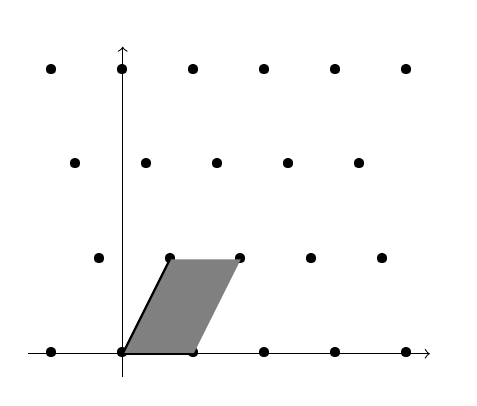
\begin{tikzpicture}[scale=0.3]
    \draw[->, thin] (-4,0)--(13,0) node [right] {}; 
    \draw[->, thin] (0,-1)--(0,13) node [above] {};
    \foreach \Point in {(-3,0), (0,0), (3,0), (6,0), (9,0), (12,0), (-1,4), (2,4), (5,4), (8,4), (11,4), (-2,8), (1,8), (4,8), (7,8), (10,8), (-3,12), (0,12), (3,12), (6,12), (9,12), (12,12)}{
        \node at \Point {\textbullet};    
    }
    \path[fill=gray] (0,0)--(3,0)--(5,4)--(2,4)--(0,0);
    \draw[thick] (0,0)--(3,0);
    \draw[thick] (0,0)--(2,4);
    \end{tikzpicture}
    $$
    \caption{The fundamental domain for the lattice generated by $\lbrace (3,0), (2,4) \rbrace$.}
\end{figure}

Fundamental domains have many interesting properties. One essential property to note is that the volume of a lattice's fundamental domain is an invariant. To see this property, we first define a unimodular matrix. 
\begin{defn}
    A square matrix $\mathbf{U}$ of integer entries is \textit{unimodular} if $|\text{det}(\mathbf{U})|=1$.
\end{defn}

The crux of this paper, as we will see, lies in the idea that multiple bases can generate the same lattice. Given a basis $\B$, we refer to its matrix representation by $\mathbf{B}$, so that 
$$\mathbf{B} = 
\begin{bmatrix}
    \mathbf{b_0}\\
    \mathbf{b_1}\\
    \vdots\\
    \mathbf{b_{n-1}}
\end{bmatrix}.
$$

Now, we will formalize the condition that allows two bases to generate the same lattice. This condition has to do with the concept of a unimodular matrix. 

\begin{thm}
    For two bases $\B_{0},\B_{1}$ for $\R^n$, $\LA(\B_0)=\LA(\B_1)$ if and only if there exists a unimodular matrix $\mathbf{U}$ such that $\mathbf{B}_{0} = \mathbf{B}_{1}\mathbf{U}$.
\end{thm}

\begin{proof}
    Proof adapted from Theorem 2 of \cite{MicciancioLec2}.
    
    Let two bases $\B_{0},\B_{1}$ for $\R^n$ be given. Observe that if $\mathbf{U}$ is unimodular, then so is $\mathbf{U}^{-1}$. First, suppose that $\mathbf{B}_{0} = \mathbf{B}_{1}\mathbf{U}$ for some unimodular $\mathbf{U}$. Since $\mathbf{B}_{0} = \mathbf{B}_{1}\mathbf{U}$, by the definition of a lattice it follows that $\LA(\B_0) \subset \LA(\B_1)$. Since $\mathbf{B}_{1} = \mathbf{B}_{0}\mathbf{U}^{-1}$, by the definition of a lattice it follows that $\LA(\B_1) \subset \LA(\B_0)$. 
    
    Now, we prove the other direction. Suppose that $\LA(\B_1) = \LA(\B_0)$. Then, by the definition of a lattice, there exists square integer matrices $\mathbf{M}, \mathbf{N}$ such that $\mathbf{B}_{0} = \mathbf{B}_{1}\mathbf{N}$ and $\mathbf{B}_{1} = \mathbf{B}_{0}\mathbf{M}$. It follows that $\mathbf{B}_{0}(\mathbf{I} - \mathbf{N}\mathbf{M}) = \mathbf{0}$, where $\mathbf{I}$ is the identity matrix. Since the row vectors of $\mathbf{B}_{0}$ are linearly independent, it follows that $\mathbf{I} = \mathbf{N}\mathbf{M}$. Hence, $$\text{det}(\mathbf{N}\mathbf{M}) =  \text{det}(\mathbf{N})\text{det}(\mathbf{M}) = \text{det}(\mathbf{I}) = 1.$$ Since the entries of $\mathbf{N}, \mathbf{M}$ are integers, it follows that $$|\text{det}(\mathbf{N})| = |\text{det}(\mathbf{M})| = 1.$$
\end{proof}

We now define the determinant of a lattice. 

\begin{defn}\label{determinant}
    For any lattice $\LA(\B)$, we define the \textit{determinant} of that lattice to be $\text{det}(\LA(\B)) := \text{Vol}(\mathcal{F}(\B) = \prod_{i=0}^{n-1}\|\ba_{i}^{*}\|$.
\end{defn}

Next, we prove a different representation of the determinant of a lattice. 

\begin{thm}
    For any basis $\B$, we can express $\text{det}(\LA(\B))$ as $$\text{det}(\LA(\B)) = \sqrt{\text{det}(\mathbf{B}^{T}\mathbf{B})}.$$
\end{thm}

\begin{proof}
    Proof adapted from Theorem 6 of \cite{MicciancioLec2}.

    Consider some basis $\B$. Consider also the Gram-Schmidt orthogonalization $\B^*$ and the corresponding matrix $\mathbf{B}^*$. Observe that, by the Gram-Schmidt Algorithm, there is an upper triangular matrix $\mathbf{T}$ with all $1$s on the main diagonal and the coefficients $\frac{\langle\ba_{j}^{*},\ba_{i}\rangle}{\langle\ba_{j}^{*},\ba_{j}^{*}\rangle}$ at the position $\mathbf{T}_{ji}$ for all $j < i$, such that $\mathbf{B} = \mathbf{B}^{*}\mathbf{T}$. Thus, we can write 
    \begin{align*} 
        \sqrt{\text{det}(\mathbf{B}^{T}\mathbf{B})} &= \sqrt{\text{det}(\mathbf{B}^{T}(\mathbf{B}^{*}\mathbf{T}))} \\
        &= \sqrt{\text{det}((\mathbf{T}^{T}\mathbf{B}^{*T})(\mathbf{B}^{*}\mathbf{T}))} \\
        &= \sqrt{\text{det}(\mathbf{T}^{T})\text{det}(\mathbf{B}^{*}^{T}\mathbf{B}^{*})\text{det}(\mathbf{T}))}.
    \end{align*} 
    Since $\mathbf{T},\mathbf{T}^T$ are triangular matrices, both $\text{det}(\mathbf{T}),\text{det}(\mathbf{T}^{T})$ are the products of their respective diagonal entries. So, $\text{det}(\mathbf{T}^{T}) = \text{det}(\mathbf{T}^{T}) = 1$. Since both $\mathbf{B}, \mathbf{B}^*$ have orthogonal columns, the matrix $\mathbf{B}^{*}\mathbf{B}$ is diagonal. Hence, $\text{det}(\mathbf{B}^{*}\mathbf{B})$, is the product of the diagonal entries of $\mathbf{B}^{*}\mathbf{B}$. Thus, $$\text{det}(\mathbf{B}^{*T}\mathbf{B}^{*}) = \prod_{i=0}^{n-1}\langle\ba_{i}^{*},\ba_{i}^{*}\rangle = \prod_{i=0}^{n-1}\|\ba_{i}^{*}\|^2 = \text{det}(\LA)^2,$$ and so 
    \begin{align*}
        \sqrt{\text{det}(\mathbf{B}^{T}\mathbf{B})} &= \sqrt{\text{det}(\mathbf{T}^{T})\text{det}(\mathbf{B}^{*}^{T}\mathbf{B}^{*})\text{det}(\mathbf{T}))} \\ 
        &= \sqrt{\text{det}(\mathbf{B}^{*T}\mathbf{B}^{*})} \\
        &= \text{det}(\LA).
    \end{align*}
\end{proof}

We are now ready to prove that the volume of a lattice's fundamental domain is an invariant, using the previous few results. 

\begin{thm}
    For any two bases $\B_{0}, \B_{1}$, if $\LA(\B_{0})) = \LA(\B_{1}))$, then $$\text{det}(\LA(\B_{0})) = \text{det}(\LA(\B_{1})).$$
\end{thm}

\begin{proof}
    Proof adapted from Theorem 7 of \cite{MicciancioLec2}.

    Consider two bases $\B_{0}, \B_{1}$ such that $\LA(\B_{0})) = \LA(\B_{1}))$. By Theorem 3.2.3, there exists a unimodular matrix $\mathbf{U}$ such that $\mathbf{B}_{0} = \mathbf{B}_{1}\mathbf{U}$. By Theorem 3.2.5, and since $\text{det}(\mathbf{U}) = \text{det}(\mathbf{U}^{T}) = 1$ we have that 
    \begin{align*}
        \text{det}(\LA(\B_{0})) &= \sqrt{\text{det}(\mathbf{B}_{0}^{T}\mathbf{B}_{0})} \\
        &= \sqrt{\text{det}(\mathbf{B}_{0}^{T}(\mathbf{B}_{1}\mathbf{U}))} \\
        &= \sqrt{\text{det}((\mathbf{U}^{T}\mathbf{B}_{1}^{T})(\mathbf{B}_{1}\mathbf{U}))} \\
        &= \sqrt{\text{det}(\mathbf{U}^{T})\text{det}(\mathbf{B}_{1}^{T}\mathbf{B}_{1})\text{det}(\mathbf{U})} \\
        &= \sqrt{\text{det}(\mathbf{B}_{1}^{T}\mathbf{B}_{1})} \\
        &= \text{det}(\LA(\B_{1})).
    \end{align*}
\end{proof}

Thus, we have shown that every fundamental domain of a lattice has the same volume.
Another interesting property to note is the relationship between the volume of a lattice's fundamental domain and a measure of the orthogonality of its basis. This relationship is represented by the Hadamard Inequality. 

\begin{defn}\label{Hadamard}
For any lattice $\LA(\B)$, the \textit{Hadamard Inequality} states that  
$$\text{det}(\LA)) \leq \prod_{i=0}^{n-1}\| \ba_i \|.$$
\end{defn}

Equality is achieved only when the given basis is orthogonal. We use the term \textit{Hadamard ratio} to refer to the ratio $$\frac{\prod_{i=0}^{n-1}\| \ba_i \|}{\text{det}(\LA)}.$$

This makes sense by noting that since the basis vectors form the sides of the fundamental domain, the volume of the fundamental domain is maximized precisely when the basis vectors are orthogonal to one another. 

A crucial aspect of the fundamental domain is that it provides a tiling of $\R^n$.

\begin{thm}
    For any basis $\B$, a given vector $\mathbf{w} \in \R^n$ can be expressed uniquely as the sum $\mathbf{f} + \mathbf{v}$ for a pair $\mathbf{f} \in \mathcal{F}(\B)$, $\mathbf{v} \in \LA(\B)$.
    \begin{figure}[H]
        $$
            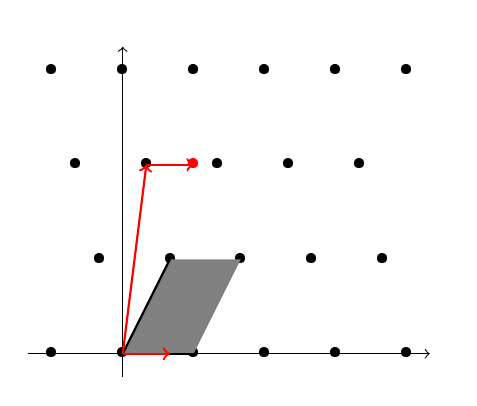
\begin{tikzpicture}[scale=0.3]
                \draw[->, thin] (-4,0)--(13,0) node [right] {}; 
                \draw[->, thin] (0,-1)--(0,13) node [above] {};
                \foreach \Point in {(-3,0), (0,0), (3,0), (6,0), (9,0), (12,0), (-1,4), (2,4), (5,4), (8,4), (11,4), (-2,8), (1,8), (4,8), (7,8), (10,8), (-3,12), (0,12), (3,12), (6,12), (9,12), (12,12)}{\node at \Point {\textbullet};}
                \path[fill=gray] (0,0)--(3,0)--(5,4)--(2,4)--(0,0);
                \node [red] at (3,8) {\textbullet};
                \draw[thick] (0,0)--(3,0);
                \draw[thick] (0,0)--(2,4);
                \draw[->, thick, red] (0,0)--(1,8);
                \draw[->, thick, red] (1,8)--(3,8);
                \draw[->, thick, red] (0,0)--(2,0);
            \end{tikzpicture}
        $$
        \caption{Any real vector is the sum of a unique pair of one lattice vector and one vector in the fundamental domain.}
    \end{figure}
\end{thm}

\begin{proof}
    Proof adapted from Proposition 7.18 in \cite{HPS}. 
    
    Fix some basis $\B = \lbrace \ba_0, \ba_1,...,\ba_{n-1}\rbrace$. Let some $\mathbf{w} \in \R^n$ be given. Since the vectors $\ba_0,\ba_1,...,\ba_{n-1}$ are linearly independent, they generate $\R^n$. So, we can write $$\mathbf{w} = \alpha_0\ba_0 + \alpha_1\ba_1 + ... + \alpha_{n-1}\ba_{n-1}$$ for some $\lbrace \alpha_i \rbrace \subset \R$. We can further express each $\alpha_i$ as $\alpha_i = f_i + v_i$ for some $f_i \in [0,1), v_i \in \mathbb{Z}$. So, 
    \begin{align*}
        \mathbf{w} &= (f_0 + v_0)\ba_0 + ... + (f_{n-1} + v_{n-1})\ba_{n-1} \\
                   &= (f_0\ba_0 + ... + f_{n-1}\ba_{n-1}) + (v_0\ba_0 + ... + v_{n-1}\ba_{n-1}).
    \end{align*}
    Note that $$\mathbf{f} = f_0\ba_0 + ... + f_{n-1}\ba_{n-1} \in \mathcal{F}(\B),$$ $$\mathbf{v} = v_0\ba_0 + ... + v_{n-1}\ba_{n-1} \in \LA(\B),$$ giving us the existence of the desired pair of vectors so that $\mathbf{w} = \mathbf{f} + \mathbf{v}$. Now, we show uniqueness. Suppose $\mathbf{w} = \mathbf{e} + \mathbf{u}$, where $$\mathbf{e} = {e_0}\ba_0 + ... + e_{n-1}\ba_{n-1} \in \mathcal{F}(\B),$$ $$\mathbf{u} = u_0\ba_0 + ... + u_{n-1}\ba_{n-1} \in \LA(\B),$$ and $\lbrace e_i \rbrace \subset [0,1)$, $\lbrace u_i \rbrace \subset \mathbb{Z}$.  Then, since $\ba_0, ..., \ba_{n-1}$ are linearly independent, we have that $$f_i + v_i = e_i + u_i$$ for all $0 \leq i \leq n-1$. Hence, for each $i$, $f_i - e_i = u_i - v_i \in \mathbb{Z}$. Since each $f_i,e_i \in [0,1)$, we must have that $f_i - e_i = 0$. So, $u_i - v_i = 0$. Thus, $\mathbf{f} = \mathbf{e}$ and $\mathbf{v} = \mathbf{u}$, as desired. 
\end{proof}

\subsection{Successive Minima}

It can be useful to consider not only the shortest nonzero distance of a lattice, but also the second shortest nonzero distance, the third shortest, and so on. We refer to these as the successive minima of a lattice, and denote them as $\lambda_{0}(\LA)$, $\lambda_{1}(\LA)$, $\lambda_{2}(\LA)$, $\lambda_{3}(\LA)$,...,$\lambda_{n-1}(\LA)$. The successive minima of a lattice are defined similarly to the minimum distance of a lattice, and a similar argument as the one above shows that they are in fact achieved by lattice vectors. We now present a few results which will build toward providing an upper bound for the successive minima of a lattice. The first of these theorems, Blichfeld's Theorem, makes a statement on the determinant of a lattice. 

\begin{thm}\label{Blichfeld}
    For any lattice $\LA(\B)$ and measurable set $S \subset \R^n$ with $\text{Vol}(S) > \text{det}(\LA)$, there are two distinct $\mathbf{z_1},\mathbf{z_2} \in S$ such that $\mathbf{z_1} - \mathbf{z_2} \in \LA$. 
\end{thm}
 
\begin{proof}
    Proof adapted from Theorem 8 in \cite{RegevIntro}.
    
    Consider some lattice $\LA(\B)$ and measurable set $S \subset \R^n$. By Theorem 3.1.9, the translates of $\mathcal{F}(\B)$ partition $\R^n$. For $\mathbf{x}\in \LA$, let $$S_\mathbf{x} = S \cap (\mathbf{x} + \mathcal{F}(\B)), \hat{S}_\mathbf{x} = S_\mathbf{x} - \mathbf{x}.$$ Since $S = \bigcup_{\mathbf{x}\in\LA}S_\mathbf{x}$, we have that $$\text{Vol}(S) = \sum_{\mathbf{x}\in\LA}\text{Vol}(S_\mathbf{x}).$$ Note that $\hat{S}_\mathbf{x} \subset \mathcal{F}(\B)$ and $\text{Vol}(\hat{S}_\mathbf{x}) = \text{Vol}(S_\mathbf{x})$. Thus, 
    \begin{align*}
        \sum_{\mathbf{x}\in\LA}\text{Vol}(\hat{S}_\mathbf{x}) &= \sum_{\mathbf{x}\in\LA}\text{Vol}(S_\mathbf{x}) \\
        &= \text{Vol}(S) \\
        &> \text{Vol}(\mathcal{F}(\B)).
    \end{align*}
    Therefore, there must be distinct $\mathbf{z_{1}},\mathbf{z_{2}} \in \LA$ such that $\hat{S}_\mathbf{z_1} \cap \hat{S_\mathbf{z_2}} \neq \varnothing$. Pick some $\mathbf{z} \in \hat{S}_\mathbf{z_1} \cap S_\mathbf{z_2}$. Note that $$\mathbf{z} + \mathbf{z_1} \in S_\mathbf{z_1} \subset S, \mathbf{z} + \mathbf{z_2} \in S_\mathbf{z_2} \subset S.$$ Thus, $(\mathbf{z}+\mathbf{z_1})-(\mathbf{z}+\mathbf{z_2}) = \mathbf{z_1}-\mathbf{z_2} \in \LA$, as desired.
\end{proof}

Before discussing the results of Blichfeld's Theorem, we provide a few definitions from geometry. 

\begin{defn}
    A set is $S \subset \R^n$ is \textit{centrally symmetric} if for any $\mathbf{x}\in S$, there also exists $\mathbf{-x} \in S$.
\end{defn}

\begin{defn}
    A set $S \subset \R^n$ is \textit{convex} if for any $\mathbf{x},\mathbf{y}\in S$ and $\alpha \in [0,1]$, there also exists $\alpha \mathbf{x} + (1-\alpha)\mathbf{y} \in S$.
\end{defn}

As a result of Blichfeld's Theorem, we attain the following corollary due to Minkowski, which is called the Convex Body Theorem. 

\begin{thm}
    For any lattice $\LA(\B)$ and centrally symmetric convex set $S \subset \R^n$, if $\text{Vol}(S) > 2^{n}\text{det}(\LA)$ then $S$ contains a nonzero $\mathbf{v} \in \LA$.
\end{thm}

\begin{proof}
    Proof adapted from Theorem 9 in \cite{RegevIntro}.
    
    Consider some lattice $\LA(\B)$ and centrally symmetric convex set $S \subset \R^n$ such that $\text{Vol}(S) > 2^{n}\text{det}(\LA)$. Let $\hat{S} = \frac{1}{2}S$. Note that $$\text{Vol}(\hat{S}) = 2^{-n}\text{Vol}(S) > \text{det}(\LA).$$ Then, by Blichfeld's Theorem, there are two distinct $\mathbf{z_{1}},\mathbf{z_{2}} \in \hat{S}$ such that $\mathbf{z_{1}}-\mathbf{z_{2}} \in \LA$. By construction, $2\mathbf{x_{1}},2\mathbf{z_{2}} \in S$. Since $S$ is centrally symmetric, $-2\mathbf{x_{2}} \in S$. Since $S$ is convex, $\frac{2\mathbf{z_{1}} - 2\mathbf{z_{2}}}{2} = \mathbf{z_{1}}-\mathbf{z_{2}} \in S$, as desired. 
\end{proof}

We are now ready to show a bound for the minimum distance and the successive minima of a lattice. The following corollary is called Minkowski's First Theorem. 

\begin{thm}
    For any lattice $\LA(\B)$, $\lambda_{0}(\LA) \leq \sqrt{n}(\text{det}(\LA))^{1/n}$.
\end{thm}

\begin{proof}
    Proof adapted from Corollary 2 in \cite{RegevIntro}.
    
    Consider some lattice $\LA(\B)$. We denote the open neighborhood of radius $a$ centered at $b$ by $\mathcal{N}_{a}(b)$.
    Let $\epsilon > 0$. Consider the cube $$X = \Big\lbrace \mathbf{x}\in\R^n \mid |x_{i}| < \frac{2\epsilon}{n}, 0\leq i\leq n-1 \Big\rbrace ,$$ where we write $\mathbf{x} = (x_0, x_1,...,x_{n-1})$. Note that $X \subset \mathcal{N}_{\epsilon}(0)$, and that each side of $X$ has length $\frac{2\epsilon}{\sqrt{n}}$. Thus, $\text{Vol}(\mathcal{N}_{\epsilon}(0)) \geq \frac{2\epsilon}{\sqrt{n}}^n$. Also note that $\LA \cap \mathcal{N}_{\lambda_{0}(\LA)}(0) = \varnothing$. By the Convex Body Theorem, $$\frac{(2\lambda_{0}(\LA))^n}{(\sqrt{n})^n} \leq \text{Vol}(\mathcal{N}_{\lambda_{0}(\LA)}(0)) \leq 2^{n}\text{det}(\LA).$$ It follows that $\lambda_{0}(\LA) \leq \sqrt{n}(\text{det}(\LA))^{1/n}$, as desired.
\end{proof}

The following result, called Minkowski's Second Theorem, strengthens the bound given by Minkowski's First Theorem by giving a bound that considers the geometric mean of all successive minima $\lambda_i, 0\leq i\leq n-1$.

\begin{thm}
    For any lattice $\LA(\B)$, $$\Big(\prod_{i=0}^{n-1}\lambda_{i}(\LA)\Big)^{1/n} \leq \sqrt{n}(\text{det}(\LA))^{1/n}.$$
\end{thm}

\begin{proof}
    Proof adapted from Theorem 3 of \cite{RegevIntro}.
    
    Consider some lattice $\LA(\B)$. Let $X = \lbrace\mathbf{x}_0, \mathbf{x}_1, ..., \mathbf{x}_{n-1}\rbrace \subset \LA$ be a basis for $\R^n$ such that each $\|\mathbf{x}_{i}\| = \lambda_{i}(\LA)$. Let $X^*$ be the Gram-Schmidt orthogonalization of $X$. Consider the open ellipsoid $E$ with axes $\mathbf{x_0}^{*}, \mathbf{x_1}^{*}, ..., \mathbf{x_{n-1}}^{*}$: $$E = \Big\lbrace \mathbf{y} \in \R^n \mid \sum_{i=0}^{n-1}\Big(\frac{\langle\mathbf{y},\mathbf{x_i}^*\rangle}{\|\mathbf{x_i}^{*}\|\lambda_{i}(\LA)}\Big)^{2} < 1  \Big\rbrace.$$
    We will first show that $E$ does not contain any nonzero lattice vector. Pick some nonzero $\mathbf{w} \in \LA$ and the largest index $k$ such that $\|\mathbf{w}\| \geq \lambda_{k}(\LA)$. By our choice of $X$, it follows that $\mathbf{w} \in \mathcal{S}(\lbrace\mathbf{x}_{0}^{*},...,\mathbf{x}_{k}^{*}\rbrace)$. Observe that \begin{align*}
        \sum_{i=0}^{n-1}\Big(\frac{\langle\mathbf{w},\mathbf{x_i}^*\rangle}{\|\mathbf{x_i}^{*}\|\lambda_{i}(\LA)}\Big)^{2} &= \sum_{i=0}^{k}\Big(\frac{\langle\mathbf{w},\mathbf{x_i}^*\rangle}{\|\mathbf{x_i}^{*}\|\lambda_{i}(\LA)}\Big)^{2} \\
        &\geq \sum_{i=0}^{n-1}\Big(\frac{\langle\mathbf{w},\mathbf{x_i}^*\rangle}{\|\mathbf{x_i}^{*}\|\lambda_{k}(\LA)}\Big)^{2} \\ 
        &= \lambda_{k}(\LA)^{-2}\sum_{i=0}^{n-1}\Big(\frac{\langle\mathbf{w},\mathbf{x_i}^*\rangle}{\|\mathbf{x_i}^{*}\|}\Big)^{2} \\
        &= \frac{\|\mathbf{w}\|^{2}}{\lambda_{k}(\LA)^{2}} \\
        &\geq 1.
    \end{align*}
    Thus, $\mathbf{w} \notin E$. Now, by the Convex Body Theorem, $$\text{Vol}(E) \geq 2^{n}\text{det}(\LA).$$ We also have that $$\text{Vol}(E) = \Big(\prod_{i=0}^{n-1}\lambda_{i}\Big)\text{Vol}(\mathcal{N}_{1}(0)) \geq \Big(\prod_{i=0}^{n-1}\lambda_{i}\Big)\Big(\frac{2}{\sqrt{n}}\Big)^{n}.$$ Therefore, $$\Big(\prod_{i=0}^{n-1}\lambda_{i}\Big)\Big(\frac{2}{\sqrt{n}}\Big)^{n} \leq 2^{n}\text{det}(\LA),$$ i.e. $$\Big(\prod_{i=0}^{n-1}\lambda_{i}\Big)^{1/n} \leq \sqrt{n}\text{det}(\LA)^{1/n}.$$
\end{proof}

We have thus far introduced a linear algebraic concept of lattices. This definition is convenient for use in computer science. At the same time, it can also be helpful to look at lattices geometrically. We will reconcile the linear algebraic and geometric definitions of lattices.

\begin{defn}\label{second def of lattices}
    A \textit{discrete additive subgroup} of $\R^n$ is an additive subgroup $\mathcal{G}$ of $\R^n$ such that for all $\mathbf{v} \in \mathcal{G}$, there exists $\epsilon \in \R$ such that 
    $$\lbrace \mathbf{w} \in \mathcal{G} \mid \|\mathbf{v} - \mathbf{w}\| < \epsilon \rbrace = \lbrace \mathbf{v} \rbrace.$$
\end{defn}

\begin{thm} \label{equivalent definitions}
For any subset $L \subset \R^n$, the following statements are equivalent.
\begin{enumerate}
    \item $L = \left\{ \sum_{i=0}^{n-1} x_{i}\ba_{i} \mid x_{i} \in \mathbb{Z} \right\}$ for some basis $\B = \lbrace\ba_0, \ba_1, ..., \ba_{n-1}\rbrace$.
    \item $L$ is a discrete additive subgroup of $\R^n$.
\end{enumerate}

\end{thm}

In proving Theorem 3.1.10, we will use the concept of a closed fundamental domain.

\begin{defn}\label{closed fd}
    For any basis $\B$, we define the \textit{closed fundamental domain} of $\LA(\B)$ to be the set $$\overline{\mathcal{F}}(\B) := \left\{ \sum_{i=0}^{n-1} x_{i}\ba_{i} \mid 0 \leq x_{i} \leq 1 \right\}.$$
\end{defn}

We now proceed to the proof of Theorem 3.1.10.

\begin{proof}
Let $\B \subset \R^n$ be a set of linearly independent vectors $\ba_0, \ba_1, ..., \ba_{n-1}$ generating a subset $L \subset \R^n$. Since $L$ is the set of all integer linear combinations of $\B$, for any vectors $\sum_{i=0}^{n-1} x_{i}\ba_{i} \text{ and } \sum_{i=0}^{n-1} y_{i}\ba_{i}$ in $L$ we have that $$\sum_{i=0}^{n-1} (x_{i} + y_{i})\ba_i , \sum_{i=0}^{n-1} (-x_{i})\ba_i \in L.$$ Note that $\sum_{i=0}^{n-1} 0\ba_i = \mathbf{0} \in L$. Thus, $L$ is an additive subgroup of $\R^n$. Then, for any distinct $\mathbf{v}, \mathbf{w} \in L$, we must have that $\mathbf{v} - \mathbf{w} \in L$. It follows that $\| \mathbf{v} - \mathbf{w} \| \geq \lambda_{0}(L)$. Let $\epsilon = \lambda_{0}(L)$. Then, $$\lbrace \mathbf{z} \in L \mid \|\mathbf{v} - \mathbf{z}\| < \epsilon \rbrace = \lbrace \mathbf{v} \rbrace,$$ as desired. Therefore, $L$ is a discrete additive subgroup of $\R^n$. 

We have shown that Definition 3.1.3 implies Definition 3.1.10. We will now prove the opposite direction. The proof in this direction is adapted from \cite{VinodV}.

% https://people.csail.mit.edu/vinodv/COURSES/CSC2414-F11/L2.pdf

Let $L$ be a discrete additive subgroup of $\R^n$. Choose $\mathbf{y} \in L$ such that there is no $\hat{\mathbf{y}} \in L$ where $\hat{\mathbf{y}} = \alpha \mathbf{y}$ and $\alpha \in (0,1)$. Let $\ba_0 = \mathbf{y}$. We now describe a recursive method for selecting the vectors $\ba_1, \ba_2, ..., \ba_{n-1}$. 

For $0 \leq i < n-1$, suppose $\ba_0, ..., \ba_i$ have already been chosen. Choose $\mathbf{w}_i \in L$ such that $\mathbf{w}_i \notin \mathcal{S}(\lbrace \ba_0,...,\ba_i \rbrace)$. Now, consider the closed fundamental domain $\overline{\mathcal{F}}(\lbrace \ba_0,...,\ba_i,\mathbf{w}_i \rbrace)$. Notice that $\overline{\mathcal{F}}(\lbrace \ba_0,...,\ba_i,...,\mathbf{w}_i \rbrace)$ contains $\mathbf{w}_i$ and so contains at least one member of $L$. Observe that the intersection $L^{'} = L \cap \overline{\mathcal{F}}(\lbrace \ba_0,...,\ba_i,...,\mathbf{w}_i \rbrace)$ is closed, and so since $\overline{\mathcal{F}}(\lbrace \ba_0,...,\ba_i,...,\mathbf{w}_i \rbrace)$ is compact $L^'$ must also be compact. Further observe that $L^'$ is discrete. Hence, by a result of topology, $L^'$ is finite. By construction, we must have a member of $L$ in the set difference $$\overline{\mathcal{F}}_i = \overline{\mathcal{F}}(\lbrace \ba_0,...,\ba_i,\mathbf{w}_i \rbrace) \setminus \mathcal{S}(\lbrace \ba_0,...,\ba_i\rbrace).$$ 

We can express the distance from any singleton $\lbrace \alpha \rbrace$ to a set $B$ as $$\text{dist}(\lbrace\alpha\rbrace,B) = \inf\lbrace \|\alpha - \beta\| \mid \beta \in B\rbrace.$$ It is a well-known result that this distance is well-defined and is achieved by some $\beta \in B$ if $B$ is closed. Thus, since $L \cap \overline{\mathcal{F}}_i$ is compact, for any $\alpha \in L \cap \overline{\mathcal{F}}_i$ we can find $\beta_\alpha$ such that $\text{dist}(\lbrace\alpha\rbrace,B) = \|\alpha - \beta_\alpha\|$. Further, since $L \cap \overline{\mathcal{F}}_i$ is finite, we can find some  $\mathbf{w_{i+1}} \in L \cap \overline{\mathcal{F}}_i$ such that $$\text{dist}(\lbrace\mathbf{w}_{i+1}\rbrace, L \cap \overline{\mathcal{F}}_i) = \min\Big\lbrace\text{dist}(\lbrace\alpha\rbrace, \mathcal{S}(\lbrace \ba_0,...,\ba_i\rbrace)\mid \alpha \in  L \cap \overline{\mathcal{F}}_i\Big\rbrace.$$ Let $\ba_{i+1} = \mathbf{w}_{i+1}$. 

Since by construction each $\ba_{i+1} \notin \mathcal{S}(\lbrace \ba_0,...,\ba_i\rbrace)$, the vectors $\ba_0,...,\ba_{n-1}$ are linearly independent. We claim that $$L = \left\{ \sum_{i=0}^{n-1} x_{i}\ba_{i} \mid x_{i} \in \mathbb{Z} \right\}.$$

Note that each $\ba_i \in L$ and that $L$ has closure under additivity as it is an additive subgroup of $\R^n$. It follows that $$\left\{ \sum_{i=0}^{n-1} x_{i}\ba_{i} \mid x_{i} \in \mathbb{Z} \right\} \subset L.$$

Now, consider some $\mathbf{z} \in L$. Since $\ba_0,...\ba_{n-1}$ are linearly independent, they generate $\R^n$. Hence, we can write $$\mathbf{z} = \sum_{i=0}^{n-1}x_{i}\ba_{i}$$ for some $x_0,...,x_{n-1} \in \R$. We will show that, in fact, $x_0,...x_{n-1} \in \mathbb{Z}$. Consider $\mathbf{z}^{'} = \sum_{i=0}^{n-1}\lfloor x_i \rfloor\ba_i \in L$. By closure, $$\mathbf{z} - \mathbf{z}^{'} = \sum_{i=0}^{n-1}(x_{i} - \lfloor x_{i}\rfloor)\ba_i \in L.$$ Now, consider the distance  $$\text{dist}(\lbrace\mathbf{z}-\mathbf{z}^{'}\rbrace, \mathcal{S}(\lbrace\ba_0,...,\ba_{n-2}\rbrace).$$ Notice that this distance equals $(x_{n-1}-\lfloor x_{n-1}\rfloor)\|\ba_{n-1}^{*}\|$, which is the orthogonal component of the vector from $\mathbf{z} - \mathbf{z}^'$ to the closest point in $\mathcal{S}(\lbrace \ba_0,...,\ba_{n-2}\rbrace)$. Thus, we have that $$\text{dist}(\lbrace\mathbf{z}-\mathbf{z}^{'}\rbrace, \mathcal{S}(\lbrace\ba_0,...,\ba_{n-2}\rbrace) = (x_{n-1}-\lfloor x_{n-1}\rfloor)\|\ba_{n-1}^{*}\|.$$ Similarly, $$\text{dist}(\lbrace\ba_{n-1}\rbrace, \mathcal{S}(\lbrace\ba_0,...,\ba_{n-2}\rbrace) = \|\ba_{n-1}^*\|.$$ Since $0 \leq x_{n-1}-\lfloor x_{n-1}\rfloor < 1$, we have that $$(x_{n-1}-\lfloor x_{n-1}\rfloor)\|\ba_{n-1}^{*}\| < \|\ba_{n-1}^{*}\|.$$ However, recall that by construction $\ba_{n-1}$ is the closest member of $L$ to $\mathcal{S}(\lbrace\ba_0,...,\ba_{n-2})$. Therefore, $x_{n-1}-\lfloor x_{n-1}\rfloor = 0$ and so $x_{n-1} \in \mathbb{Z}$. We repeat this strategy for all $x_{n-2},...x_0$ to find that all the coefficients $x_i$ are integers. Thus, $\mathbf{z} \in \left\{ \sum_{i=0}^{n-1} x_{i}\ba_{i} \mid x_{i} \in \mathbb{Z} \right\}$ and so $L \subset \left\{ \sum_{i=0}^{n-1} x_{i}\ba_{i} \mid x_{i} \in \mathbb{Z} \right\}$, as desired.
% $$\min\big\lbrace \|\mathbf{z}-\mathbf{z}^{'}-\mathbf{v}\|\mid\mathbf{v}\in \mathcal{S}(\lbrace\ba_0,...,\ba_{n-2})\big\rbrace < \min\big\lbrace \|\mathbf{\ba_{n-1}}-\mathbf{v}\|\mid\mathbf{v}\in \mathcal{S}(\lbrace\ba_0,...,\ba_{n-2})\big\rbrace.$$
\end{proof}

We will primarily use the linear algebraic definition of lattices going forward. 

\subsection{Computational Problems} 
Any mathematical problem that is very difficult to solve without a crucial piece of information makes a good candidate for a cryptosystem. Lattice-based cryptosystems are based on two optimization problems thought to be intractable, namely the Closest Vector Problem (CVP) and the Shortest Vector Problem (SVP). The crux of the CVP is to find the lattice vector closest to a given vector. The crux of the SVP is to find the shortest vector of a given lattice, i.e. the to find the lattice vector whose length is $\lambda_{0}(\LA)$. We first introduce the two problems formally, and then we discuss their connection to the lattice properties which we have introduced.

\begin{defn}\label{CVP}
Given a lattice $\LA(\B)$ and a vector $\mathbf{w} \in \R^n$, the \textit{Closest Vector Problem (CVP)} for $(\LA, \mathbf{w})$ is to find some $\mathbf{v} \in \LA$ that minimizes $\| \mathbf{v} - \mathbf{w} \|$. 
\end{defn}

\begin{defn}\label{SVP}
Given a lattice $\LA(\B)$, the \textit{Shortest Vector Problem (SVP)} for $\LA$ is to find some nonzero $\mathbf{v} \in \LA$ that minimizes $\| \mathbf{v} \|$.
\end{defn}

Note that there may be multiple shortest vectors or closest vectors, which is why the problems ask not for \textit{the} vector but for \textit{some} vector. The SVP can be considered to be a variant of the CVP, as in the SVP we are tasked with finding the closest nonzero lattice vector to the origin. The SVP varies from the CVP in this regard only by the inclusion of the word "nonzero", as solving the CVP given the origin yields the origin itself. These two problems are considered to be extremely computationally difficult, and their difficulty grows with the dimension of the given lattice. In fact, the CVP has been shown to be $\mathcal{NP}$-difficult \cite{Dinur}. The SVP has been shown to be no harder than the CVP \cite{Goldreich}, though under certain conditions it also is $\mathcal{NP}$-difficult \cite{AjtaiSVP}. However, as the dimension grows, it is also harder to form an efficient cryptosystem based on these problems as it becomes increasingly computationally taxing to encrypt information. Hence, in practice, we are usually more interested in approximation variants of the SVP and CVP. 

A naive yet straightforward approach to finding a shortest vector in the lattice is determining the shortest basis vector. This approach tends to have good results when dealing with a "nice" basis, i.e. an orthogonal or near-orthogonal basis. However, there is no guarantee that the approach will yield a satisfactory result when dealing with a "bad" basis, i.e. a far from orthogonal basis.

\begin{figure}[H]
    \centering
    \begin{subfigure}{.5\textwidth}
        $$
        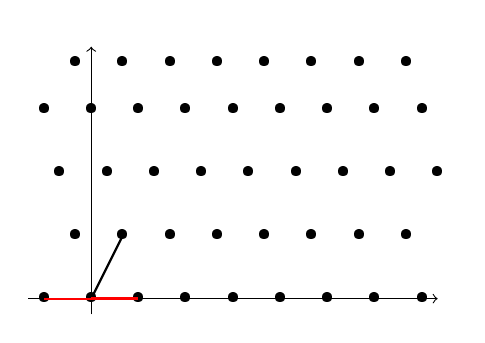
\begin{tikzpicture}[scale=0.2]
        \draw[->, thin] (-4,0)--(22,0) node [right] {}; 
        \draw[->, thin] (0,-1)--(0,16) node [above] {};
        \foreach \Point in {(-3,0), (0,0), (3,0), (6,0), (9,0), (12,0), (15,0), (18,0), (21,0), (-1,4), (2,4), (5,4), (8,4), (11,4), (14,4), (17,4), (20,4), (-2,8), (1,8), (4,8), (7,8), (10,8), (13,8), (16,8), (19,8), (22,8), (-3,12), (0,12), (3,12), (6,12), (9,12), (12,12), (15,12), (18,12), (21,12), (-1,15), (2,15), (5,15), (8,15), (11,15), (14,15), (17,15), (20,15)}{
            \node at \Point {\textbullet};    
        }
        \draw[thick] (0,0)--(3,0);
        \draw[thick] (0,0)--(2,4);
        \draw[style=very thick, color=red] (0,0)--(3,0);
        \draw[thick, color=red] (0,0)--(-3,0);
        \end{tikzpicture}
        $$
        \caption{$\B_0 = \lbrace (3,0), (2,4) \rbrace$}
    \end{subfigure}%
    \begin{subfigure}{.5\textwidth}
        $$
        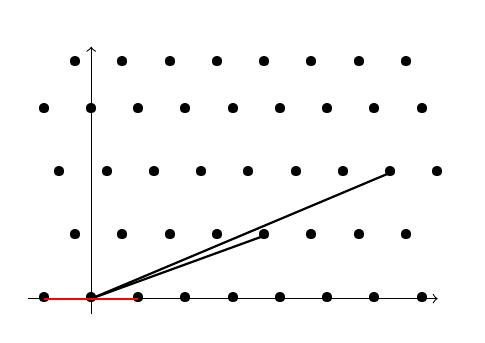
\begin{tikzpicture}[scale=0.2]
        \draw[->, thin] (-4,0)--(22,0) node [right] {}; 
        \draw[->, thin] (0,-1)--(0,16) node [above] {};
        \foreach \Point in {(-3,0), (0,0), (3,0), (6,0), (9,0), (12,0), (15,0), (18,0), (21,0), (-1,4), (2,4), (5,4), (8,4), (11,4), (14,4), (17,4), (20,4), (-2,8), (1,8), (4,8), (7,8), (10,8), (13,8), (16,8), (19,8), (22,8), (-3,12), (0,12), (3,12), (6,12), (9,12), (12,12), (15,12), (18,12), (21,12), (-1,15), (2,15), (5,15), (8,15), (11,15), (14,15), (17,15), (20,15)}{
            \node at \Point {\textbullet};    
        }
        \draw[thick] (0,0)--(19,8);
        \draw[thick] (0,0)--(11,4);
        \draw[thick, color=red] (0,0)--(3,0);
        \draw[thick, color=red] (0,0)--(-3,0);
        \end{tikzpicture}
        $$
        \caption{$\B_1 = \lbrace (11,4), (19,8) \rbrace$} 
    \end{subfigure}%
    \caption{The set of shortest vectors (marked in red) from the origin of the lattice generated by $\B_0$ includes the shortest basis vector $(3,0)$. The same cannot be said for $\B_1$.}
\end{figure}

\begin{ex}
    Consider a lattice generated by $\B_0 = \lbrace (3,0), (2,4) \rbrace$. The Hadamard ratio for $\B_0$ is $\frac{\|(3,0)\|\|(2,4)\|}{12} = \frac{3 \times 2\sqrt{5}}{12} \approx 1.12$. Though this basis is not orthogonal, it is close enough to being orthogonal that the shortest basis vector, $(3,0)$, is a shortest lattice vector along with $(-3,0)$.
\end{ex}
\begin{ex}
    The same lattice as in the previous example can be generated by $\B_1 = \lbrace (11,4), (19,8) \rbrace$, since
    \begin{align*}
       2(11,4) - (19,18) &= (3,0), \\ -5(11,4) + 3(19,8) &= (2,4), \\ 3(3,0) + (2,4) &= (11,4), \\ 5(3,0) + 2(2,4) &= (19,8). 
    \end{align*}
However, the  Hadamard ratio for $\B_1$ is $\frac{\|(11,4)\|\|(19,8)\|}{40} = \frac{\sqrt{137}\times\sqrt{425}}{40} \approx 6.03$. The set of shortest vectors here does not contain the shortest basis vector, $(11,4)$. So, computing the shortest vector of $\LA(\B_1)$ is a more complex problem than simply surveying the basis for a vector of minimum length.
\end{ex}

 See Figure 4 for an illustration of the preceding examples. We have begun to see how having a "nice" basis would be beneficial for breaking a cryptosystem based on the SVP. 

In the following chapters, we discuss algorithms aimed at solving the SVP and the CVP. We also develop an understanding of the desirability for orthogonal bases.

\newpage

% ************************************************************************
% Babai's Closest Vertex Algorithm
% ************************************************************************
\section{Babai's Closest Vertex Algorithm}\label{Babai}

The most common approach to solve the CVP is to use Babai's Closest Vertex Algorithm. In this chapter we introduce the algorithm and consider examples that illustrate how the success of the algorithm is contingent on the choice of basis. This chapter draws considerably from Section 7.6 in \cite{HPS}.

Suppose we want to solve the CVP for a given lattice $\LA(\B)$ and vector $\mathbf{w} \in \R^n$, where $\B$ is orthogonal. Since $\B$ spans $\R^n$, we can write $$\mathbf{w} = \sum_{i=0}^{n-1} a_{i}\ba_{i}$$ for some $a_0, a_1, ..., a_{n-1} \in \R$. Then, for any lattice vector $\mathbf{v} = \sum_{i=0}^{n-1} x_{i}\ba_{i}$, it follows that $$\| \mathbf{v} - \mathbf{w} \|^2 = \sum_{i=0}^{n-1} (x_i - a_i)^{2}\|\mathbf{\ba}_i\|^2.$$ 

We can see that to solve the CVP for $(\LA, \mathbf{w})$, we must minimize the sum of $(x_i - a_i)^2$ over all $i$. Since each $x_i$ is an integer, each individual difference $|x_i - a_i|$ is minimized if $x_i = \lfloor a_i \rceil$, where we denote the nearest integer to $a_i$ by $\lfloor a_i \rceil$. Recall that, by Theorem 3.2.8, the translates of $\mathcal{F}(\B)$ by lattice vectors tile $\R^n$. So, $\mathbf{w}$ is contained in some unique translate $\mathcal{F}(\B) + \mathbf{z} \subset \R^m$. The vertex of the translate $\mathcal{F}(\B) + \mathbf{z}$ closest to $\mathbf{w}$ is a candidate for a solution to the CVP. See Figure 5 for an illustration.

The method described above tends to be successful only when the given basis is "nice", i.e. orthogonal or near-orthogonal. The method does not work when the given basis is "bad", i.e. far from orthogonal. 

\begin{defn}
For any lattice $\LA(\B)$ and vector $\mathbf{w} \in \R^n$, \textit{Babai's Closest Vertex Algorithm} is as follows: 
{
\fontfamily{cmss}\selectfont
$$\fbox{
\begin{varwidth}{\textwidth}
    \text{Find} $\lbrace a_i \rbrace \subset \R$ \text{such that} $\mathbf{w} = \sum_{i=0}^{n-1} a_{i}\ba_i$. \\
    \text{Loop} $i = 0, ..., n-1$. \\ 
    \text{  \, \,    Set } $x_i = \lfloor a_i \rceil$. \\
    \text{End Loop.} \\
    \text{Return} $\mathbf{v} = \sum_{i=0}^{n-1} x_{i}\ba_i$.
\end{varwidth} 
}$$ 
}
\end{defn}

\begin{figure}[H]
    $$
    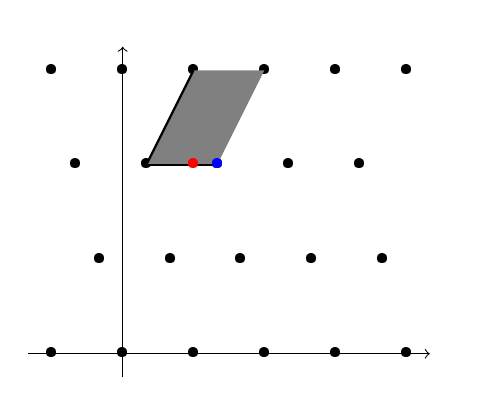
\begin{tikzpicture}[scale=0.3]
    \draw[->, thin] (-4,0)--(13,0) node [right] {}; 
    \draw[->, thin] (0,-1)--(0,13) node [above] {};
    %\draw[dotted] (-1,-1) grid (3,3);
    \foreach \Point in {(-3,0), (0,0), (3,0), (6,0), (9,0), (12,0), (-1,4), (2,4), (5,4), (8,4), (11,4), (-2,8), (1,8), (4,8), (7,8), (10,8), (-3,12), (0,12), (3,12), (6,12), (9,12), (12,12)}{
        \node at \Point {\textbullet};    
    }
    \path[fill=gray] (1,8)--(4,8)--(6,12)--(3,12)--(1,8);
    \draw[thick] (1,8)--(4,8);
    \draw[thick] (1,8)--(3,12);
    \node[color=red] at (3,8) {\textbullet};
    \node[color=blue] at (4,8) {\textbullet};
    \end{tikzpicture}
    $$
    \caption{For the target vector $(3,8)$, the vertex $(4,8)$ of the unique translate $\mathcal{F}(\B) + (1,8)$ is our candidate to solve the CVP.}
\end{figure}

We consider two examples of the algorithm demonstrating varying levels of success. See Figure 6 for an illustration.

\begin{ex}
Suppose we are given a basis $\B_0 = \lbrace (3,0), (2,4) \rbrace$ and a vector $\mathbf{w} = (3,8)$. Recall from Example 2.2.3 that the Hadamard ratio for $\B_0$ is approximately 1.12. We wish to solve the CVP for $(\LA(B_0), \mathbf{w})$. We can express $\mathbf{w}$ as a linear combination $(3,8) = a_{1}(3,0) + a_{2}(2,4)$. We can solve the system to find $a_1 = -\frac{1}{3}$, $a_2 = 2$ and thus $x_1 = 0$, $x_2 = 2$. This yields the lattice vector $\mathbf{v} = 0(3,0) + 2(2,4) = (4,8)$. We find that $\| \mathbf{v} - \mathbf{w} \| = 1$. Given a near orthogonal basis, we have found the closest lattice vector to $\mathbf{w}$.  
\end{ex}

\begin{ex}
Suppose we are given a basis $\B_1 = \lbrace (11,4), (19,8) \rbrace$ and a vector $\mathbf{w} = (3,8)$. By Example 3.4.4, $\B_1$ generates the same lattice as $\B_0$ did in Example 4.0.2. Recall from Example 2.2.4 that the Hadamard ratio for $\B_0$ is approximately 6.03. We wish to solve the CVP for $(\LA(B_1), \mathbf{w})$. We can express $\mathbf{w}$ as a linear combination $(3,8) = a_{1}(11,4) + a_{2}(19,8)$. We can solve the system to find $a_1 = -\frac{32}{3}$, $a_2 = \frac{19}{3}$ and thus $x_1 = -11$, $x_2 = 6$. This yields the lattice vector $\mathbf{v} = -11(11,4) + 6(19,8) = (-7,4)$. We find that $\| \mathbf{v} - \mathbf{w} \| = \sqrt{116} \approx 10.77$. Given a basis that is far from being orthogonal, we have found a lattice vector quite far from $\mathbf{w}$. 
\end{ex}

\begin{figure}[H]
    \centering
    \begin{subfigure}{.5\textwidth}
        $$
        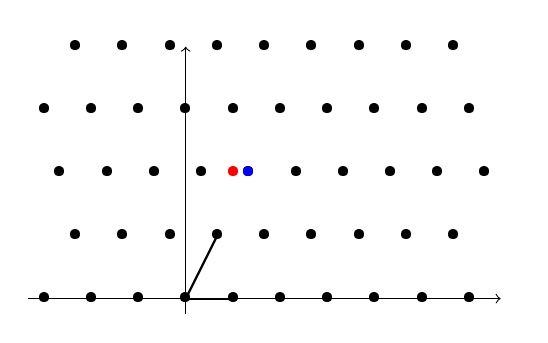
\begin{tikzpicture}[scale=0.2]
        \draw[->, thin] (-10,0)--(20,0) node [right] {}; 
        \draw[->, thin] (0,-1)--(0,16) node [above] {};
        \foreach \Point in {(-9,0), (-6,0), (-3,0), (0,0), (3,0), (6,0), (9,0), (12,0), (15,0), (18,0), (-7,4), (-4,4), (-1,4), (2,4), (5,4), (8,4), (11,4), (14,4), (17,4), (-8,8), (-5,8), (-2,8), (1,8), (4,8), (7,8), (10,8), (13,8), (16,8), (19,8), (-9,12), (-6,12), (-3,12), (0,12), (3,12), (6,12), (9,12), (12,12), (15,12), (18,12), (-7,16), (-4,16), (-1,16), (2,16), (5,16), (8,16), (11,16), (14,16), (17,16)}{
            \node at \Point {\textbullet};    
        }
        \node[color=red] at (3,8) {\textbullet};
        \node[color=blue] at (4,8) {\textbullet};
        \draw[thick] (0,0)--(3,0);
        \draw[thick] (0,0)--(2,4);
        \end{tikzpicture}
        $$
        \caption{$\B_0 = \lbrace (3,0), (2,4) \rbrace$}
    \end{subfigure}%
    \begin{subfigure}{.5\textwidth}
        $$
        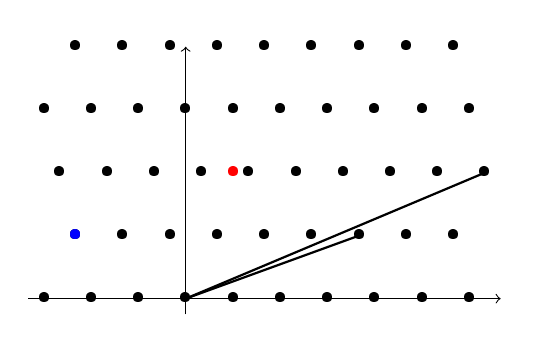
\begin{tikzpicture}[scale=0.2]
        \draw[->, thin] (-10,0)--(20,0) node [right] {}; 
        \draw[->, thin] (0,-1)--(0,16) node [above] {};
        \foreach \Point in {(-9,0), (-6,0), (-3,0), (0,0), (3,0), (6,0), (9,0), (12,0), (15,0), (18,0), (-7,4), (-4,4), (-1,4), (2,4), (5,4), (8,4), (11,4), (14,4), (17,4), (-8,8), (-5,8), (-2,8), (1,8), (4,8), (7,8), (10,8), (13,8), (16,8), (19,8), (-9,12), (-6,12), (-3,12), (0,12), (3,12), (6,12), (9,12), (12,12), (15,12), (18,12), (-7,16), (-4,16), (-1,16), (2,16), (5,16), (8,16), (11,16), (14,16), (17,16)}{
            \node at \Point {\textbullet};    
        }
        \node[color=red] at (3,8) {\textbullet};
        \node[color=blue] at (-7,4) {\textbullet};
        \draw[thick] (0,0)--(19,8);
        \draw[thick] (0,0)--(11,4);
        \end{tikzpicture}
        $$
        \caption{$\B_1 = \lbrace (11,4), (19,8) \rbrace$} 
    \end{subfigure}%
    \caption{Target vectors marked red and the output of Babai's algorithm marked blue. The algorithm works well for near orthogonal bases like $\B_1$ but poorly for far from orthogonal bases like $\B_1$.}
\end{figure}

Let us discuss the intuition behind this variability in the success of Babai's Closest Vertex Algorithm. The algorithm works by first finding the translate of $\mathcal{F}(\B)$ containing the given vector $\mathbf{w}$. Call this translate $\mathcal{F} + \mathbf{t}$. Next, it finds the closest vertex of $\mathcal{F} + \mathbf{t}$ to $\mathbf{w}$. When $\B$ is "nice", the vertices of $\mathcal{F}(\B)$ are relatively close to each other. So, the closest lattice vector to $\mathbf{w}$ must be one of the vertices of $\mathcal{F} + \mathbf{t}$. When $\B$ is "bad", however, the vertices of $\mathcal{F}(\B)$ are relatively far from each other; thus, the algorithm overlooks several lattice vectors in its attempt to find the closest vertex of $\mathcal{F} + \mathbf{t}$ to $\mathbf{w}$. In our working example, given the "bad" basis $\lbrace (11,4), (9,8)\rbrace$, the algorithm overlooks vectors such as $(4,8), (1,8), (2,4), (-1,4)$, et cetera, that are close to $(3,8)$ and settles for the translate's closest vertex $(-7,4)$.

From our discussion up to now, we have seen that a "nice" basis is desirable when attempting to solve the SVP or the CVP. The following chapters will focus on algorithms that aim to replace a given basis with a more suitable one; we know that it is possible to do so and still generate the same lattice by Theorem 3.2.3.

\newpage

% ************************************************************************
% Lagrange's Reduction Algorithm
% ************************************************************************
\section{Lagrange's Reduction Algorithm}\label{Lagrange}

There are many lattice reduction algorithms, all aiming to transform any given basis into a "nice" basis. Each algorithm has its own definition of what constitutes a "nice" basis, but a common goal is to produce basis vectors which are short and near orthogonal. In two dimensions, the algorithm for finding a lattice's optimal basis is due to Lagrange. It is often misattributed to Gauss, who described the same procedure later. In this section, we will present Lagrange's Reduction Algorithm along with an example. This will be an appropriate introduction for the next chapter, which will discuss a generalization of Lagrange's Reduction Algorithm to higher dimensions: the LLL algorithm. 

% cite https://perso.ens-lyon.fr/damien.stehle/downloads/lowdim-final.pdf

Recall the Gram-Schmidt Algorithm which we introduced in Definition 3.1.2. One might wonder why we don't simply utilize the Gram-Schmidt Algorithm if we wish to have an orthogonalized basis. After all, while we are looking for algorithms to return a near-orthogonal basis, here lies an algorithm which returns an orthogonal basis. The issue with using the Gram-Schmidt Algorithm is that the projection coefficients $\frac{\langle \mathbf{\ba_{i-1}^*}, \mathbf{\ba_i} \rangle}{\langle \mathbf{\ba_{i-1}^*}, \mathbf{\ba_{i-1}^*} \rangle}$ are not necessarily integers. Thus, the resulting vectors in $\B^*$ do not necessarily lie in the given lattice. 

Since the Gram-Schmidt Algorithm is not enough when dealing with lattices, we instead focus here on the Lagrange Reduction Algorithm. This algorithm produces what we call a Lagrange-reduced basis, which is the first type of a "nice" basis that we consider. 

\begin{defn}
A basis $\B = \lbrace \ba_0, \ba_1 \rbrace \subset \R^2$ is \textit{Lagrange-reduced} if it satisfies the following conditions:
    \begin{enumerate}
    \item $\|\ba_0\| \leq \|\ba_1\|$.
    \item $\frac{| \langle \ba_1, \ba_0 \rangle |}{\langle \ba_0, \ba_0 \rangle} \leq \frac{1}{2}$.
    \end{enumerate}
\end{defn}

We can refer to these two properties as saying that the basis is \textit{ordered} and \textit{near-orthogonal}, respectively. Note that the fraction in the second property is the coefficient in $\mu_{\ba_0}(\ba_1)$, As the basis vectors become closer to being orthogonal, this coefficient gets smaller. In fact, when the vectors are orthogonal, this coefficient equals $0$. 

A Lagrange-reduced basis is handy not just for rendering Babai's Closest Vertex Algorithm useful, but also for solving the SVP in dimension 2.

\begin{thm}
If a basis $\B \subset \R^2$ is Lagrange-reduced, then $\ba_0$ is a shortest vector of $\LA(\B)$.  
\end{thm}

\begin{proof}
Proof adapted from Proposition 7.66 of \cite{HPS}. 

    Let $\B \subset \R^2$ be a Lagrange-reduced basis. Then, we have that 
    \begin{align}
        \|\ba_0\| \leq \|\ba_1\|, \\
        \frac{| \langle \ba_0, \ba_1 \rangle |}{\langle \ba_0, \ba_0 \rangle} \leq \frac{1}{2}.
    \end{align} 
    Let $\mathbf{v} \in \LA(\B)$ such that  $\|\mathbf{v}\| = \lambda_{0}(\LA(\B))$ be given. This means that $\mathbf{v}$ is a shortest vector of $\LA(\B)$. (Recall that a lattice may have multiple shortest vectors.) We will show that $\|\ba_0\| = \|\mathbf{v}\|$.
    
    We can express the given shortest vector as $\mathbf{v} = x_{0}\ba_0 + x_{1}\ba_1$ for some integers $x_0, x_1$. Since $\B$ is Lagrange-reduced, it follows that 
    \begin{align*}
    \|\mathbf{v}\|^2 &= \|x_0\ba_0 + x_1\ba_1\|^2 \\
                     &= x_0^2\|\ba_0\|^2 + x_1^2\|\ba_1\|^2 + 2x_0x_1\langle \ba_0, \ba_1 \rangle \\
                     &\geq x_0^2\|\ba_0\|^2 + x_1^2\|\ba_1\|^2 - 2|x_0x_1|\langle\ba_0, \ba_1 \rangle \\
                     &\geq x_0^2\|\ba_0\|^2 + x_1^2\|\ba_1\|^2 - |x_0x_1|\langle\ba_0, \ba_0 \rangle \text{\,\,\,\,\,\,\,\,by (2)} \\ 
                     &\geq x_0^2\|\ba_0\|^2 + x_1^2\|\ba_0\|^2 - |x_0x_1|\langle\ba_0,\ba_0 \rangle \text{\,\,\,\,\,\,\,\,\,\,by (1)} \\
                     &= (x_0^2 + x_1^2 - |x_0x_1|)\|\ba_0\|^2.
    \end{align*}
    Note that $x_0^2 + x_1^2 - |x_0x_1| = 0$ only when $x_0 = x_1 = 0$. Since $x_0,x_1$ are integers, it follows that $$(x_0^2 + x_1^2 - |x_0x_1|)\|\ba_0\|^2 \geq \|\ba_0\|^2.$$ Thus, $\|\mathbf{v}\|^2 \geq \|\ba_0\|^2$. Since $\ba_0 \in \LA(\B)$ and $\mathbf{v}$ is a shortest vector of the lattice, it must be that $\|\mathbf{v}\| = \|\ba_0\|$. Therefore, $\ba_0$ is a shortest vector of $\LA(\B)$.
\end{proof}

Thus, finding a Lagrange-reduced basis for a given lattice in dimension 2 can solve the SVP. 

The time is ripe to examine Lagrange's Reduction Algorithm. Any basis for a subset of $\R^2$ consists of two basis vectors. The idea behind Lagrange's Reduction Algorithm is to create a Lagrange-reduced basis by subtracting multiples of one basis vector from the other basis vector until no improvement is possible. By Theorem 3.2.3, multiple bases can generate the same lattice. That result ensures the validity of Lagrange's Reduction Algorithm, which improves a given basis and produces another basis that generates the same lattice. There are two main steps in the algorithm: a \textit{swap} step and a \textit{reduction} step, which ensure that the output of the algorithm abides by the two properties of a Lagrange-reduced basis. 

\begin{defn}
For any lattice $\LA(\B) \subset \R^2$, \textit{Lagrange's Reduction Algorithm} is as follows:
{
\fontfamily{cmss}\selectfont
$$\fbox{
\begin{varwidth}{\textwidth}
    \text{Set} $\ba^\prime_{0} = \ba_0, \ba^\prime_1 = \ba_1$. \\
    \text{Loop} \\
    \text{  \, \, If} $\|\ba^\prime_0\| > \|\ba^\prime_1\|$ \\
    \text{  \, \, \, \, Swap} $\ba^\prime_0, \ba^\prime_1$. \\
    \text{  \, \, Compute } $m = \Big\lfloor \frac{\langle\ba_0^{'},\ba_1^{'}\rangle}{\langle\ba_0^{'},\ba_0^{'}\rangle} \Big\rceil$. \\
    \text{  \, \, If } $m = 0$ \\ 
    \text{  \, \, \, \, Break Loop}. \\
    \text{  \, \, Set } $\ba^\prime_1 = \ba^\prime_1 - m\ba_0^'$. \\
    \text{Return } $\B^\prime = \lbrace \ba^\prime_0, \ba^\prime_1 \rbrace$. \\    
\end{varwidth}
} 
$$ 
}
\end{defn}

For a proof for the termination of the algorithm, refer to Proposition 3.1 in \cite{Tian} . The key point to note is that the value $\min\lbrace\|\ba_{0},\ba_{1}\|\rbrace$ decreases note is that on each iteration of the algorithm, and so the projection coefficient (which is the length of the projection) also decreases and is eventually rounded to the nearest integer $0$.

Notice that Lagrange's Reduction Algorithm basis is Lagrange-reduced. Swapping ensures that $\|\ba_0^{'}\| < \|\ba_1^{'}\|$, and reducing $\ba_1^{'}$ by $m\ba_0^{'}$ ensures that $\frac{| \langle \ba_0^{'}, \ba_1^{'} \rangle |}{\langle \ba_0^{'}, \ba_0^{'} \rangle} \leq \frac{1}{2}$. Let us now consider an example. 

\begin{ex}
Suppose we are given a basis $\B = \lbrace(11,4), (19,8)\rbrace$. We apply Lagrange's Reduction Algorithm to $\B$. 
\begin{enumerate}
    \item We set $\ba_0^{'} = (11,4), \ba_1^{'} = (19,8)$.
    \item Since $\|\ba_0^{'}\| = \|\sqrt{137}\| < \|\ba_1^{'}\| = \sqrt{425}$, we do not swap.
    \item We compute $m = \lfloor\frac{209+32}{137}\rceil = 2$. So, we set $$\ba_1^{'} = (19,8) - 2(11,4) = (-3,0).$$
        \begin{figure}[H]
            $$
            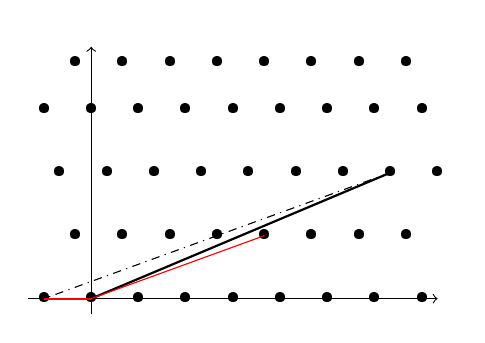
\begin{tikzpicture}[scale=0.2]
            \draw[->, thin] (-4,0)--(22,0) node [right] {}; 
            \draw[->, thin] (0,-1)--(0,16) node [above] {};
            \foreach \Point in {(-3,0), (0,0), (3,0), (6,0), (9,0), (12,0), (15,0), (18,0), (21,0), (-1,4), (2,4), (5,4), (8,4), (11,4), (14,4), (17,4), (20,4), (-2,8), (1,8), (4,8), (7,8), (10,8), (13,8), (16,8), (19,8), (22,8), (-3,12), (0,12), (3,12), (6,12), (9,12), (12,12), (15,12), (18,12), (21,12), (-1,15), (2,15), (5,15), (8,15), (11,15), (14,15), (17,15), (20,15)}{
                \node at \Point {\textbullet};    
            }
            \draw[thick] (0,0)--(19,8);
            \draw[red] (0,0)--(11,4);
            \draw[dash dot] (19,8)--(8,4);
            \draw[dash dot] (8,4)--(-3,0);
            \draw[thick, color=red] (0,0)--(-3,0);
            \end{tikzpicture}
            $$
            \caption{The lattice generated by $\lbrace(11,4), (19,8)\rbrace$. In Step 3, the shorter basis vector $(11,4)$ is subtracted twice from the longer basis vector $(19,8)$ to yield the vector $(-3,0)$. The new values are $\ba_0^{'} = (11,4), \ba_1^{'} = (-3,0)$, marked in red.}
        \end{figure}
    \item Since $\|\ba_0^{'}\| = \|\sqrt{137}\| > \|\ba_1^{'}\| = \sqrt{9}$, we swap. Now, $$\ba_0^{'} = (-3,0), \ba_1^{'} = (11,4).$$
    \item We compute $m = \lfloor\frac{-33+0}{9}\rceil = -4$. So, we set 
    $$\ba_1^{'} = (11,4) - (-4(-3,0)) = (-1,4).$$
        \begin{figure}[H]
            $$
            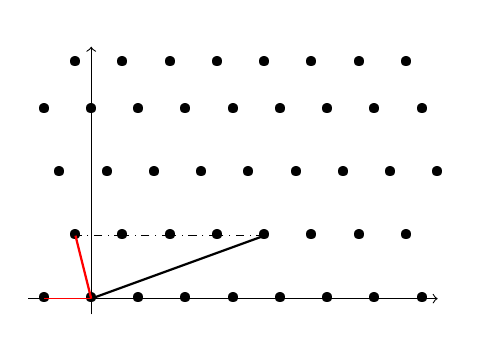
\begin{tikzpicture}[scale=0.2]
            \draw[->, thin] (-4,0)--(22,0) node [right] {}; 
            \draw[->, thin] (0,-1)--(0,16) node [above] {};
            \foreach \Point in {(-3,0), (0,0), (3,0), (6,0), (9,0), (12,0), (15,0), (18,0), (21,0), (-1,4), (2,4), (5,4), (8,4), (11,4), (14,4), (17,4), (20,4), (-2,8), (1,8), (4,8), (7,8), (10,8), (13,8), (16,8), (19,8), (22,8), (-3,12), (0,12), (3,12), (6,12), (9,12), (12,12), (15,12), (18,12), (21,12), (-1,15), (2,15), (5,15), (8,15), (11,15), (14,15), (17,15), (20,15)}{
                \node at \Point {\textbullet};    
            }
            \draw[red] (0,0)--(-3,0);
            \draw[thick] (0,0)--(11,4);
            \draw[dash dot] (11,4)--(8,4);
            \draw[dash dot] (8,4)--(5,4);
            \draw[dash dot] (5,4)--(2,4);
            \draw[dash dot] (2,4)--(-1,4);
            \draw[thick, color=red] (0,0)--(-1,4);
            \end{tikzpicture}
            $$
            \caption{The lattice generated by $\lbrace(-3,0), (11,4)\rbrace$. Note that the lattice is invariant throughout the algorithm despite the changing basis vectors. In Step 5, the shorter basis vector $(-3,0)$ is subtracted four times from the longer basis vector $(11,4)$ to yield the vector $(-1,4)$. The new values are $\ba_0^{'} = (-3,0), \ba_1^{'} = (-1,4)$, marked in red.}
        \end{figure}
    \item Since $\|\ba_0^{'}\| = \|\sqrt{9}\| < \|\ba_1^{'}\| = \sqrt{17}$, we do not swap.
    \item We compute $m = \lfloor\frac{3+0}{9}\rceil = 0$. So, we return $\B^{'} = \lbrace(-3,0),(-1,4)\rbrace$.
\end{enumerate}
Note that $(-3,0)$ is a shortest vector of $\LA(\B)$, as we demonstrated in Example 3.2.3. Thus, the algorithm easily solves the SVP for the given lattice in dimension 2.
\end{ex}

Lagrange's Reduction Algorithm is an important introduction to the LLL Algorithm, which can be thought of a rough generalization of the two dimensional algorithm to higher dimensions. In practice, lattice cryptosystems in dimension 2 are easy to break by applying Lagrange's Reduction Algorithm. This makes lattices in dimension 2 highly impractical. It is far more common to encounter lattices in higher dimensions. So, we reserve a deeper algorithmic analysis of time complexity, applications, etc. for the LLL Algorithm. 

\newpage

% ************************************************************************
% The LLL Algorithm
% ************************************************************************
\section{The LLL Algorithm}\label{LLL}

As the dimension $n$ increases, it becomes increasingly challenging to solve the SVP. It is unclear how to construct a perfect analogue of the Lagrange Reduction Algorithm in higher dimensions because of several issues. Firstly, it is uncertain what the right combination of preceding vectors $\ba_0, \ba_1, ..., \ba_{i-1}$ is with which to reduce $\ba_i$; this is straightforward to do in the dimension 2 case since for any basis vector there is only one other basis vector by which it can be reduced. Secondly, in higher dimensions it requires many more computations to order a basis as each basis vector must be compared with multiple vectors.

In 1982, Lenstra, Lenstra, and Lov\'asz published a new basis reduction algorithm \cite{LLL}. Their algorithm, which we call the LLL Algorithm, was originally aimed at factoring polynomials over $\mathbb{Q}$. The algorithm has many applications in combinatorics and number theory, such as approximating the minimal polynomial of an algebraic number, and integer programming with a fixed number of variables \cite{Lenstra}. In cryptography, there are many known LLL-based attacks on knapsack cryptosystems and RSA cryptosystems \cite{May}. 

In this chapter, we discuss the algorithm's usefulness with for solving the SVP and CVP for lattices. First, we introduce the concept of an LLL-reduced basis. Then, we present the algorithm. Finally, we provide an example and analyze the algorithm's complexity.

Recall that we denote the $i$-th basis vector as $\ba_i$ and the $i$-th Gram-Schmidt vector as $\ba_i^*$.

\begin{defn}
For $\frac{1}{4} \leq \delta < 1$, a basis $\B$ is \textit{$\delta$-LLL-reduced} if it satisfies the following conditions: 
\begin{enumerate}
    \item $\delta\| \ba_{i-1}^{*} \|^2 \leq \Big\| \frac{| \langle \ba_{i-1}^{*}, \ba_{i} \rangle |}{\langle \ba_{i-1}^{*}, \ba_{i-1}^{*} \rangle}\ba_{i-1}^{*} + \ba_{i}^{*} \Big\|^2$ for $1 \leq i < n$.
    % \item $\|\ba_{i}^{*}\|^2 \geq \Big (\frac{3}{4} - \Big|\frac{\langle \ba_i^{*}, \ba_{i-1}^{*} \rangle}{\langle \ba_i^{*}, \ba_i^{*} \rangle}\Big|^{2} \Big )\| \ba_{i-1}^{*} \|^2$.
    \item $\frac{| \langle \ba_j^{*}, \ba_i \rangle |}{\langle \ba_j^{*}, \ba_j^{*} \rangle} \leq \frac{1}{2}$ for $1 \leq j < i \leq n$.
\end{enumerate}
\end{defn}

Similar to the property of a Lagrange-reduced basis, the second property ensures reduction of basis vectors, and we refer to this property as saying that the basis is \textit{near-orthogonal}. For convenience, we generally use $\delta = \frac{3}{4}$ and refer to a $\frac{3}{4}$-LLL-reduced basis as an LLL-reduced basis. The value of $\delta$ plays a crucial role in the ordering of the basis. The first property, which we call the \textit{Lov\'asz condition}, serves to order the basis. $\delta$ acts as a scaling factor, ordering the basis not based on the lengths of vectors but on the scaled lengths of vectors. The scaling serves to relax the Lov\'asz condition, making it easier for a basis to qualify as LLL-reduced. So, to satisfy the Lov\'asz condition, a basis need not be perfectly ordered, i.e. a basis does not need to have the property that $\|\ba_{0}\| \leq ...\leq \|\ba_{n-1}\|$. This allows an algorithm which transforms a basis into an LLL-reduced basis to be more efficient as it only needs to check a more relaxed set of criteria. As the value of $\delta$ increases, the Lov\'asz condition becomes harder to meet. We do not allow $\delta = 1$ even though this would ensure perfect ordering; as we will see later, such a value of $\delta$ is thoroughly impractical. To see more readily the ordering present in an LLL-reduced basis, observe that from the Lov\'asz condition it follows that 
\begin{align*}
\frac{3}{4} \| \ba_{i-1}^{*} \|^2 &\leq \Big\| \frac{| \langle \ba_{i-1}^{*}, \ba_{i} \rangle |}{\langle \ba_{i-1}^{*}, \ba_{i-1}^{*} \rangle}\ba_{i-1}^{*} + \ba_{i}^{*} \Big\|^2 \\
&= \Big |\frac{\langle \ba_{i-1}^{*}, \ba_{i}\rangle}{\langle \ba_{i-1}^{*}, \ba_{i-1}^{*} \rangle}\Big|^{2}\|\ba_{i-1}^{*}\|^{2} + \| \ba_{i}^{*} \|^{2},
\end{align*}

with the equality resulting from the orthogonality of $\ba_{i-1}^{*}$ and $\ba_{i}^{*}$. Hence, 
\begin{align*}
\|\ba_{i}^{*}\|^2 &\geq \Big (\frac{3}{4} - \Big|\frac{\langle \ba_{i-1}^{*}, \ba_{i}^{*} \rangle}{\langle \ba_{i-1}^{*}, \ba_{i-1}^{*} \rangle}\Big|^{2} \Big )\| \ba_{i-1}^{*} \|^2 \\
&> \frac{1}{2}\| \ba_{i-1}^{*} \|^2.
\end{align*}

This shows how, in Regev's words, the Lov\'asz condition provides that each vector $\ba_{i}^*$ is not much shorter than the preceding vector $\ba_{i-1}^*$ \cite{Regev}. It is easy to verify that the statement $$\|\ba_{i}^{*}\|^2 \geq \Big (\frac{3}{4} - \Big|\frac{\langle \ba_{i-1}^{*}, \ba_{i}^{*} \rangle}{\langle \ba_{i-1}^{*}, \ba_{i-1}^{*} \rangle}\Big|^{2} \Big )\| \ba_{i-1}^{*} \|^2$$  implies the Lov\'asz condition as stated in Definition 6.0.1. The ordering given by the Lov\'asz condition is desirable for solving the SVP. We now introduce a theorem which gives an understanding of an LLL-reduced basis's desirability.

\begin{thm}[Proposition 1.11 in \cite{LLL}]
Let $\B$ be an LLL-reduced basis. Then, $$\|\ba_0\| \leq 2^{(n-1)/2}\|\mathbf{v}\|$$ for any $\mathbf{v} \in \LA(\B)$.
\end{thm}

\begin{proof}
Proof adapted from Proposition 1.11 in \cite{LLL}. First, we verify a lemma.

\begin{lem}
Let $\B$ be an LLL-reduced basis. Then, $\|\ba_{j}\|^2 \leq 2^{i}\|\ba_{i}^{*}\|^2$ for all $0 \leq j\leq i\leq n-1$.
\end{lem}

\begin{proof}[Proof of Lemma]
    We adapt the inductive argument from \cite{LLL}.
    
    Let $\B$ be an LLL-reduced basis. By induction, we will show that $$\|\ba_{j}^*\|^{2} \leq 2^{i-j}\|\ba_{i}^{*}\|^2$$ for all $0\leq j\leq i\leq n-1$. For the base case, let $j=0$. Then, we see that $$\|\ba_{0}^{*}\|^2 \leq 2\|\ba_{1}^{*}\|^2 \leq ... \leq 2^{n-1}\|\ba_{n-1}^{*}\|^2.$$ Now, suppose that $$\|\ba_{k}^{*}\|^2 \leq 2\|\ba_{k+1}^{*}\|^2 \leq ... \leq 2^{n-1-k}\|\ba_{n-1}^{*}\|^2.$$ It follows immediately that $$\|\ba_{k+1}^{*}\|^2 \leq 2\|\ba_{k+2}^{*}\|^2 \leq ... \leq 2^{n-k-2}\|\ba_{n-1}^{*}\|^2.$$ Thus, $\|\ba_{j}^*\|^{2} \leq 2^{i-j}\|\ba_{i}^{*}\|^2$ for all $0\leq j\leq i\leq n-1$.
    
    Let $0\leq j\leq i\leq n-1$. By the Gram-Schmidt Algorithm, $$\|\ba_{i}\|^{2} \leq \|\ba_{i}^{*}\|^{2} + \sum_{j=0}^{i-1}\frac{\langle\ba_{j}^{*},\ba_{i}\rangle^2}{\langle\ba_{j}^{*},\ba_{j}^{*}\rangle^2}\|\ba_{j}^{*}\|^{2}.$$ By the size condition of an LLL-reduced basis, 
    \begin{align*}
        \|\ba_{i}^{*}\|^{2} + \sum_{j=0}^{i-1}\frac{\langle\ba_{j}^{*},\ba_{i}\rangle^2}{\langle\ba_{j}^{*},\ba_{j}^{*}\rangle^2}\|\ba_{j}^{*}\|^{2} &\leq \|\ba_{i}^{*}\|^{2} +  \sum_{j=0}^{i-1}\frac{2^{i-j}}{4}\|\ba_{i}^{*}\|^{2} \\
        &= (1+\frac{2^{i}-2}{2})\|\ba_{i}^{*}\|^{2} \\
        &\leq 2^{i}\|\ba_{i}^{*}\|^{2}.
    \end{align*}
    Hence, $$\|\ba_{j}\|^{2} \leq 2^{j}\|\ba_{j}^{*}\|^{2} \leq 2^{i}\|\ba_{i}^{*}\|^{2}$$ for all $0\leq j\leq i\leq n-1$, as desired.
\end{proof}

We continue with the proof of Theorem 6.0.2. Consider any arbitrary nonzero $\mathbf{v} \in \LA(\B)$ and write \begin{align*}
    \mathbf{v} &= \sum_{i=0}^{n-1}x_{i}\ba_{i}\\
    &= \sum_{i=0}^{n-1}y_{i}\ba_{i}^*
\end{align*} for some $x_i \in \mathbb{Z}, y_i \in \R$. Let $k$ be the largest index such that $x_k \neq 0$. Then, by the Gram-Schmidt Algorithm, $x_k = y_k$. So, since $y_k$ is a nonzero integer, $$\|\ba_{k}^{*}\|^2 \leq y_{k}^{2}\|\ba_{k}^{*}\|^2 \leq \|\mathbf{v}\|^{2}.$$ Hence, $$2^{k}\|\ba_{k}^{*}\|^2 \leq 2^{k}\|\mathbf{v}\|^2 \leq 2^{n-1}\|\mathbf{v}\|^2.$$ Then, by the lemma, $$\|\ba_0\|^2 \leq 2^{k}\|\ba_{k}^{*}\|^2 \leq 2^{n-1}\|\mathbf{v}\|^2$$ and so $$\|\ba_0\| \leq 2^{(n-1)/2}\|\mathbf{v}\|,$$ as desired.
\end{proof}

Thus, finding an LLL-reduced basis for a lattice finds an approximate solution to the SVP within a factor of $2^{(n-1)/2}$. The LLL Algorithm, which reduces a given basis into an LLL-reduced basis, is thus an approximation algorithm for the SVP. 

\subsection{The Algorithm}
We now describe the LLL Algorithm. There are a few moving parts to keep track of. There are three objects which we need to follow.
\begin{enumerate}
    \item $\B$, the given set of basis vectors which we reduce and eventually return upon the algorithm's termination.
    \item $\B^*$, the set of Gram-Schmidt vectors.
    \item $k$, which we call the \textit{working index}. This value loops through the cardinality of the basis. The corresponding basis vector $\ba_k$, which we call the \textit{working vector}, is the vector in $\B$ which we are currently trying to reduce.
    \end{enumerate}

The algorithm broadly consists of two parts. 
\begin{enumerate}
    \item Given a basis $\B$, we subtract from the working vector $\ba_k$ appropriate integer multiples of the preceding vectors $\ba_0, \ba_1, ..., \ba_{k-1}$. These reductions are done in stages, and they ensure that the size condition is met.
    \item We decide, based on the Lov\'asz condition, whether the working vector is set as the next basis vector or whether it replaces the preceding basis vector. If the Lov\'asz condition is not met, we swap the working vector with the preceding basis vector and perform reduction again.
\end{enumerate}

Upon termination of the algorithm, every basis vector will have undergone reduction at least once. Though the basis vectors undergo many changes, the algorithm ensures that they always form a basis for the same lattice. Thus, when we calculate the Hadamard ratios to compare the orthogonality of the input basis to that of the returned basis, the value $\text{Vol}(\mathcal{F}(\B)$ is the same in both calculations.

\begin{defn}
For any lattice $\LA(\B)$, the \textit{LLL Algorithm} is as follows: 
{
\fontfamily{cmss}\selectfont
$$\fbox{
\begin{varwidth}{\textwidth}
    \text{Compute} $\B^{*}$. \\ 
    \text{Set} $k = 1$. \\
    \text{Loop while} $k\leq n-1$. \\
    \text{  \, \, Loop} $j = k-1, k-2, ..., 0$. \\
    \text{  \, \, \, \, Set} $\ba_k = \ba_k - \Big\lceil \frac{\langle\ba_j^{*},\ba_k\rangle}{\langle\ba_j^{*},\ba_j^{*}\rangle} \Big\rfloor\ba_j$. \\
    \text{  \, \, \, \, As necessary, recompute} $\B^{*}$. \\
    \text{  \, \, If } $\| \ba_k^* \|^2 \geq \Big (\frac{3}{4} - \frac{\langle \ba_{k-1}^{*}, \ba_{k} \rangle^{2}}{\langle \ba_{k-1}^{*}, \ba_{k-1}^{*} \rangle^{2}}\Big)\|\ba_{k-1}^*\|^2 $ \\ 
    \text{  \, \, \, \, Set} $k = k+1$. \\
    \text{  \, \, Else} \\ 
    \text{  \, \, \, \, Swap} $\ba_k, \ba_{k-1}$. \\ 
    \text{  \, \, \, \, As necessary, recompute} $\B^{*}$. \\
    \text{  \, \, \, \ Set } $k = \max\lbrace k-1, 1\rbrace$. \\
    \text{Return} $\B$.
\end{varwidth}
} 
$$ 
}
\end{defn}

Observe that, if the LLL Algorithm terminates, the returned basis is LLL-reduced. The $j$-loop ensures that each $\ba_k$ is reduced with regard to every preceding vector $\ba_j$, where $0 \leq j < k$, so that the size condition is met. Also, if the algorithm terminates, we have $k=n$ which means that every basis vector will have passed the Lov\'asz condition. An implementation of the LLL Algorithm can be accessed on GitHub at this \href{https://github.com/rrkane/LLL}{\underline{link}} \cite{Kane}. It is written in Python 2.7 and uses NumPy. 

We provide an example of the LLL Algorithm in Appendix 8.0.1. The example features a 3-dimensional basis in order to emphasize the LLL Algorithm's application to higher dimensions.

The astute eye sees that several computations in the example could have been avoided. For example, when $k=1$, it is unnecessary to compute $\ba_2^*$ as $\ba_2^*$ is not used in that pass of the algorithm. Such computations are included in the example for the untrained eye to fully understand the algorithm step-by-step, but this proves to be a naive implementation of the algorithm. An astute implementation is able to update the appropriate Gram-Schmidt vectors and projection operators as needed without recomputing $\B^*$ upon every change to $\B$. When dealing with very high dimensions, it is necessary to make smart configurations to the algorithm in order for the algorithm to terminate in a reasonable amount of time. In the following section, we discuss some concerns related to the running time and complexity of the LLL Algorithm.
\subsection{Complexity Analysis}
It is not immediately clear that the LLL Algorithm terminates in finitely many steps. Note that while incrementing $k$ takes the algorithm closer to termination, $k$ can be decremented when we set $k = \max\lbrace k-1, 1\rbrace$. This leads us to question whether the algorithm will ever exit the main $k$-loop and terminate. This question is resolved in the discussion on Theorem 7.71 of \cite{HPS}. In fact, Lenstra, Lenstra, and Lov\'asz show that the LLL Algorithm can terminate in polynomial time.
\begin{thm}[Proposition 1.26 in \cite{LLL}]
For a basis $\B$, let $\omega > \max(\lbrace\|\ba_{i}\|^{2}\rbrace)$. The number of arithmetic operations needed by the LLL Algorithm on $\B$ is in the order of $n^{4}log(\omega)$.
\end{thm}

\begin{proof}   
See Proposition 1.26 in \cite{LLL} for the full proof. The overall idea is as follows. Initialization of the algorithm takes a number of arithmetic operations in the order of $n^3$. Verifying the size condition requires a number of operations in the order of $n$. Verifying the Lov\'asz condition takes a number of operations in the order of $n^2$. Since the number of times that the Lov\'asz condition is checked is in the order of $n^{2}\log(\omega)$, the number of operations taken by the algorithm is in the order of $n^{3} + n + n^{2}(n^{2}\log(\omega))$ which is equivalent to the order of $n^{4}\log(\omega)$.
\end{proof}

Let us make a few remarks on the choice of $\delta$ in the algorithm. Note that the value of $\delta$, which we conventionally hold to be $\frac{3}{4}$, appears in the algorithm when we check the Lov\'asz condition. Using $\delta<1$ allows the algorithm to run in polynomial time but can squander several opportunities for reduction, since we do not swap whenever $\|\ba_k^*\|^2 < \|\ba_{k-1}^*\|^2$. The closer $\delta$ is to 1, the more difficult the condition to increment the working index becomes, thus leading to a better reduced and more orthogonal output. 

When we use $\delta = 1$, we refer to the LLL Algorithm as the \textit{optimal LLL Algorithm}, since it provides the best output. Earlier, we alluded to the fact that the optimal LLL Algorithm is impractical though it ensures perfect ordering. This is so because ensuring that the basis is perfectly ordered is a very hard problem. If $\delta = 1$, then the Lov\'asz condition is very difficult to meet; this results in the algorithm being stuck in the $k$-loop for a very long time. In fact, given current implementations and computing power, the optimal LLL Algorithm does not run in polynomial time. However, there is still much research yet to be done in this area. In 2003, Akhavi, for the first time, gave a  proof for a linear bound for the number of iterations of the optimal LLL Algorithm. 

\begin{thm}[Theorem 15 in \cite{Akhavi}]
For a basis $\B$, let $\theta > \max(\lbrace\|\ba_i\|\rbrace)$. For all constants $C > \big(\frac{2}{\sqrt{3}}\big)^{1/6}$, the number of iterations of the optimal LLL Algorithm on $\B$ is in the order of $C^{n^3}\log(\theta)$.
\end{thm}

\begin{proof}
See Theorem 15 in \cite{Akhavi} for the full proof. We omit the proof here. 
\end{proof}

To show that the optimal LLL Algorithm could run in polynomial time, all that remains to be done is to show that each iteration takes polynomial time. Since the number of iterations is linearly bounded, if each iteration were to take polynomial time then the entire algorithm would clearly run in polynomial time. However, it is still an open problem to find a polynomial bound for the running of each iteration for the optimal LLL Algorithm.

\subsection{Applying LLL to Cryptanalysis}

The LLL Algorithm has a host of applications to cryptanalysis of cryptosystems, such as GGH and NTRU, that are based on lattices. In the following section, we demonstrate the algorithm's application to knapsack cryptosystems. The algorithm easily breaks knapsack cryptosystems in low dimensions, and producing secure versions of knapsack cryptosystems requires dimensions so high that encryption becomes impractical. Thus, knapsack cryptosystems have fallen out of use. 

\newpage

% ************************************************************************
% Knapsack Cryptosystems
% ************************************************************************
\section{Knapsack Cryptosystems}\label{Knapsack}

\subsection{Basics on Public Key Cryptography}
We quickly review a few basic ideas from public key cryptography in order to develop a basic intuition without floundering in the intricate details. 

Public key cryptography is a broad system of cryptography using two sets of \textit{keys}: a \textit{public key}  which is shared with the world and a \textit{private key} which is kept secret to a person. Bob wishes to send a secret to Alice which only shee can read. Bob first comes up with his plaintext message and encrypts it using Alice's public key. He sends the ciphertext to Alice who uses her private key to decrypt it and recover the original message. If Eve intercepts the ciphertext on its way from Bob to Alice, she cannot decrypt the message because she does not have access to Alice's private key. In some cases, Eve is able to figure out Alice's private key if it has not been generated with due diligence. 

In theory, all public key cryptosystems are susceptible to \textit{brute force attacks} in which an eavesdropper attempts to decrypt the message by repeatedly guessing the private key. Such attacks are usually extremely inefficient. There is always research being done to construct newer, faster, and more powerful attack algorithms.

\subsection{The Subset-Sum Problem}

In the 1970s, Merkle and Hellman designed one of the earliest public key cryptosystems. Their cryptosystem, which we call the Merkle-Hellman cryptosystem, is based on a version of the classical knapsack problem. We first introduce the classical knapsack problem, also called the subset-sum problem.

\begin{defn}
    Given a set of weights $W = \lbrace w_0, w_1, ..., w_{n-1} \rbrace \subset \mathbb{Z}^+$ and a value $s \in \mathbb{Z}$, the \textit{subset-sum problem} is to find a subset $\lbrace w_{i_{0}}, w_{i_{1}}, ..., w_{i_{k}} \rbrace$, if one exists, such that $$\sum_{j=0}^{k} w_{i_{j}} = s,$$
    i.e. to find a subset of $W$ whose elements sum to $s$.
\end{defn}

An intuitive way to think of the subset-sum problem is the following: if a person is handed a knapsack of capacity $s$ and various items each with size $w_j$, can they fill the knapsack perfectly with a sampling of the items? We can formulate a cryptosystem based on this problem as follows:

Suppose the set $W$ is Alice's public key. Bob encrypts a message by first choosing a secret vector $x = (x_0, x_1, ..., x_{n-1})$ where each $x_i \in \lbrace 0,1 \rbrace$, and then sending the sum $s = \sum_{i=0}^{n-1} x_{i}w_{i}$ to Alice. Thus, Bob has used the set $W$ as a type of alphabet, picking which letters he wishes to send by assigning each index $i$ to a value in the set $\lbrace 0,1 \rbrace$. Alice, wishing to decrypt Bob's message, must find either $x$ or another binary vector that yields $s$. By finding a binary vector yielding $s$, Alice can find a subset of $W$, choosing the integers $w_j$ where $x_j = 1$ and discarding the integers $w_j$ where $x_j = 0$. 

Alice can employ brute force and compute every possible vector to find $x$. This approach requires a number of computations in the order of $2^n$ and is thus regarded as incredibly inefficient, though a simple observation provides a better approach that divides the exponent by 2. Consider the following, more efficient, approach, which is described by Odlyzko in \cite{Odlyzko}:

Upon receiving the sum $s$ from Bob, Alice splits the dimension $n$ into half, restricting her attention to the subsets of integer indices $$I = \Big\lbrace 0 \leq i \leq \Big\lceil\frac{n-1}{2}\Big\rfloor\Big\rbrace, J = \Big\lbrace \Big\lceil\frac{n-1}{2}\Big\rfloor < j \leq n-1 \Big\rbrace \subset \mathbb{Z}.$$
Alice generates the sets of sums $$\mathcal{I} = \Big\lbrace \sum_{i\in I}x_{i}w_{i} \mid x_i \in \lbrace 0,1 \rbrace \Big\rbrace , \mathcal{J} = \Big\lbrace s - \sum_{j\in J}x_{j}w_{j} \mid x_{j} \in \lbrace 0,1 \rbrace \Big\rbrace.$$ She then looks for an element in $\mathcal{I} \cap \mathcal{J}$. Observe that an element arises in the intersection precisely when a solution to the subset-sum problem is found, since if $$\sum_{i\in I}x_{i}w_{i} = s - \sum_{j\in J}x_{j}w_{j}$$ for some selection of $x_{i},x_{j} \in \lbrace 0,1 \rbrace$, then 
\begin{align*}
    s &= \sum_{i\in I}x_{i}w_{i} + \sum_{j\in J}x_{j}w_{j} \\
      &= \sum_{i=0}^{n-1}x_{i}w_{i}.
\end{align*}
This approach requires a number of computations in the order of $n2^{n/2}$, which is a significant reduction but still not close to practical. For a verification of this approach refer to Proposition 7.3 in \cite{HPS}. Of course, this level of difficulty in finding the vector $\mathbf{x}$ is good for protecting a message from an eavesdropping Eve. However, it is equally difficult for the intended recipient Alice unless we assume she has staggeringly more computational power than any eavesdropper. Since this is not a practical assumption, the general subset-sum problem does not generate a tenable cryptosystem. 

\subsection{The Merkle-Hellman Cryptosystem}
In the above discussion, what Alice needs to make decryption feasible is some secret information about $W$ which allows her to more easily find $\mathbf{x}$. This leads us to discuss the Merkle-Hellman Cryptosystem, which is built on an easier version of the general subset-sum problem.

\begin{defn}
    A set of positive integers $a_0, a_1, ..., a_k$ is \textit{superincreasing} if $a_i > \sum_{j=0}^{i-1}a_j$ for all $1 \leq i \leq k$.
\end{defn}

A simple example of a superincreasing set is $\lbrace 1, 2, 2^{2}, 2^{3}, ...\rbrace$. Observe that if $W$ is superincreasing, then there is a simple recursive approach for solving the subset-sum problem. Suppose Alice receives the sum $s = \sum_{i=0}^{n-1}x_{i}w_{i}$ knowing that $W$ is superincreasing. She solves for $x_{n-1}, x_{n-2}, ..., x_0$ in that order. First, she notices that $x_{n-1} = 1$ if and only if $s > \sum_{i=0}^{n-2}w_{i}$. So Alice is able to find $x_i \in \lbrace 0,1 \rbrace$ based on the sum of the preceding weights. Next, she notices that $x_{n-2} = 1$ if and only if $s - (x_{n-1}w_{n-1}) > \sum_{i=0}^{n-3}w_{i}$ and accordingly finds $x_{n-2} \in \lbrace 0,1 \rbrace$. She employs this recursive approach to find the entire vector $x$.

The Merkle-Hellman Cryptosystem is based on the superincreasing subset-sum problem, making it easy for a recipient to decrypt a message. However, it is just as easy for an eavesdropper to decrypt a message if both the recipient and the eavesdropper have access to the same information. The Merkle-Hellman Cryptosystem avoids this issue through the use of secret modular linear transformations to disguise the superincreasing $W$. Eavesdroppers will see the disguised public key $P$ and assume that it is a general knapsack, while Alice keeps the superincreasing $W$ private. Eavesdroppers are kept busy trying to solve the very difficult subset-sum problem, while Alice applies the inverse of the secret modular linear transformations to yield a superincreasing subset-sum problem. We now describe the cryptosystem in detail. There are three major portions of the cryptosystem: key generation, encryption, and decryption.

\begin{enumerate}[label*=\arabic*.]
    \item Key generation: Alice begins by generating a system to allow others to send her messages.
    \begin{enumerate}[label*=\arabic*.]
        \item Alice chooses a superincreasing $W = \lbrace w_0, w_1, ..., w_{n-1} \rbrace$ such that $w_0 > 2^n$. She also chooses positive coprime integers $A, B$ such that $B > \sum_{i=0}^{n-1}w_i$.
        \item Alice computes the vector $p = (p_0, p_1, ..., p_{n-1})$ where $$p_i = Aw_i \mod B.$$ Alice shares the public key $p$ and keeps the private key $(W,A,B)$ secret. 
    \end{enumerate}
    \item Encryption: Bob converts a plaintext message into ciphertext, which he then sends to Alice.
    \begin{enumerate}[label*=\arabic*.]
        \item A plaintext message can be easily converted to binary using ASCII encoding. Bob wishes to send a binary plaintext vector $x = (x_0, x_1, ..., x_{n-1})$, where each $x_i \in \lbrace 0,1 \rbrace$. He computes the dot product $$s = \langle x,p\rangle = \sum_{i=0}^{n-1}x_{i}p_{i}.$$ The sum $s$ is the ciphertext which he sends Alice. 
    \end{enumerate}
    \item Decryption: Alice receives a ciphertext from Bob, which she converts back into the original plaintext message.
    \begin{enumerate}[label*=\arabic*.]
        \item Alice receives $s$. Knowing $A, B$, she computes \begin{align*}
            s' &= A^{-1}s \mod B \\
            &= A^{-1}\sum_{i=0}^{n-1}x_{i}p_{i} \mod B \\
            &= A^{-1}\sum_{i=0}^{n-1}x_{i}Aw_{i} \mod B \\
            &= \sum_{i=0}^{n-1}x_{i}w_{i} \mod B.
        \end{align*}
        Here, $A^{-1}$ refers to the multiplicative inverse of $A$ modulo $B$. Now, Alice solves the subset-sum problem for $s'$ using the superincreasing $W$ and the recursive method outlined above. Since $\sum_{i=0}^{n-1}x_{i}w_{i} < \sum_{i=0}^{n-1}w_{i} < B$, which is the modulus, Alice knows that she has found an exact solution to the subset-sum problem and not a congruence. Alice recovers the vector $x$ and reads the message sent by Bob.
    \end{enumerate}
\end{enumerate}

Let us have a brief discussion on the complexity of this cryptosystem. Merkle and Hellman recommended applying several more modular operations to add additional layers of security; these recommendations are discussed at length by Odlyzko \cite{Odlyzko}. For a reasonable standard of security, we must insist that $w_0 > 2^n$. If $w_0 > 2^n$, it follows from the superincreasing nature of $W$ that the sum $s$ is in the order of $2^{2n}$. This results in the public key $p$ being quite large compared to the public keys in the RSA cryptosystem. Though the large key size is a slight inconvenience in terms of information capacity, Merkle-Hellman turns out to be significantly faster than RSA because it requires very few modular operations. Encryption requires no modular operations, and decryption requires only a few modular multiplications. Thus, Merkle-Hellman was attractive for its high speed.

However attractive the Merkle-Hellman cryptosystem was due to its speed, several doubts were raised regarding its security. Fundamental flaws in knapsack cryptosystems were uncovered in the 1980s by Shamir \cite{Shamir} and others, but these were mainly of theoretical interest. The LLL Algorithm provided a practical attack, which we now present.

\subsection{The LLL Attack on Knapsack Cryptosystems}
The following attack is described elegantly in \cite{LaO}. Suppose Bob sends an encrypted message $s$ to Alice, who has made $p$ public but has kept $(W,A,B)$ private. Unfortunately, an eavesdropping Eve intercepts the ciphertext. She can connect the subset-sum problem to lattice as follows. Eve forms an $(n+1) \times (n+1)$ matrix $$
\begin{bmatrix}
    1& 0& \cdots& 0& p_0\\
    0& 1& \cdots& 0& p_1\\
    \vdots& \vdots& \ddots& \vdots& \vdots\\
    0& 0& \cdots& 1& p_{n-1}\\
    0& 0& \cdots& 0& -s
\end{bmatrix},
$$and constructs a lattice basis $\B$ with the rows of the matrix, assigning $ 
\ba_0 = (1, 0, \ldots, 0, p_0),
\ba_1 = (0, 1, \ldots, 0, p_1),
$ and so on. Thus Eve generates $\LA(\B) \subset \R^{n+1}$. Eve wants to recover the vector $x$. She considers the lattice vector 
\begin{align*}
    X &= \sum_{i=0}^{n-1}x_{i}\ba_{i} - \ba_{n} \\
    &= (x_0, x_1, \ldots, x_n, 0).
\end{align*} Note that this vector is quite short, since each $x_i \in \lbrace 0,1 \rbrace$. So, there is a good chance that $X$ solves the SVP for $\LA(\B)$. Thus, we can transform the subset-sum problem into a problem with which we are now very familiar. We can utilize the LLL Algorithm to find the shortest vector of the lattice $\mathcal{L}(\B)$, and this vector has a high chance of being $X$. Lagarias and Odlyzko have found that for almost all problems where $\frac{n}{\log_{2}\max\lbrace p_i\rbrace} < 0.645$, the vector $X$ does indeed solve the SVP \cite{LaO}. Further, they found that for almost all problems where $\frac{n}{\log_{2}\max\lbrace p_i\rbrace} < \frac{1}{n}$, the first basis vector of the LLL-Reduced basis is in fact $X$. Such problems where the value $\frac{n}{\log_{2}\max\lbrace p_i\rbrace}$ is quite low are called problems of \textit{low density}. Even if the LLL Algorithm does not return $X$, Eve can apply the algorithm nonetheless and find $X$ in the LLL-reduced basis $\B$. Having found $X$, Eve can easily recover $x$. Let us provide a short example in which the algorithm does not return $X$ but includes $X$ in the returned basis.

\begin{ex}
    Example adapted from \cite{Bakker}. 
    
    Alice chooses the superincreasing set $W = \lbrace 2,5,9,21,45,103,215,450,946\rbrace$ and the coprime $A=1289, B=2003$. These make up her private key. Notice that $2003 > 1796 = \sum_{i=0}^{8}w_i$. She computes the vector \begin{align*}
        p &= 1289(2,5,9,21,45,103,215,450,946) \mod 2003 \\
        &= (575, 436, 1586, 1030, 1921, 569, 721, 1183, 1570),
    \end{align*} which she shares as her public key. Suppose Bob wishes to send Alice the binary message $x = (1,0,1,1,0,0,1,1,1)$. He encrypts the message by computing the sum $s = \langle x,p\rangle = 6665$, which he sends to Alice. Suppose this message is intercepted by the eavesdropping Eve, who wishes to recover $x$ from $s$. All Eve knows is the public key $p$ and the ciphertext $s$. Eve forms the matrix 
    $$
    \begin{bmatrix}
        1& 0& 0& 0& 0& 0& 0& 0& 0& 575\\
        0& 1& 0& 0& 0& 0& 0& 0& 9& 436\\
        0& 0& 1& 0& 0& 0& 0& 0& 0& 1586\\
        0& 0& 0& 1& 0& 0& 0& 0& 0& 1030\\
        0& 0& 0& 0& 1& 0& 0& 0& 0& 1921\\
        0& 0& 0& 0& 0& 1& 0& 0& 0& 569\\
        0& 0& 0& 0& 0& 0& 1& 0& 0& 721\\
        0& 0& 0& 0& 0& 0& 0& 1& 0& 1183\\
        0& 0& 0& 0& 0& 0& 0& 0& 1& 1570\\
        0& 0& 0& 0& 0& 0& 0& 0& 0& -6665\\
    \end{bmatrix}
    $$
    and forms $\B$ by letting $\ba_0$ be the first row of the matrix, and so on. Applying the LLL Algorithm to $\B$ yields the LLL-reduced basis with vectors  
    \begin{align*}
        \ba_0 =& ( -2,-1,1,0,0,0,0,0,0,0), \\
        \ba_1 =& ( 0,0,0,-1,0,1,-1,1,0,1), \\ 
        \ba_2 =& ( 1,-1,0,-2,1,0,0,0,0,0), \\ 
        \ba_3 =& ( 0,1,-1,-1,1,0,2,-1,0,0), \\ 
        \ba_4 =& ( 1,-1,-1,1,0,2,-1,0,0,0), \\ 
        \ba_5 =& ( 0,0,-1,0,1,0,-1,-1,1,1), \\ 
        \ba_6 =& ( 1,0,1,1,0,0,1,1,1,0), \\ 
        \ba_7 =& ( -1,-1,0,1,-1,0,1,1,0,2), \\ 
        \ba_8 =& ( -2,0,-1,0,-1,0,1,2,1,0), \\
        \ba_9 =& ( 1,1,0,-1,-2,0,1,0,2,0).
    \end{align*} 
    It is trivial for Eve to scan the LLL-reduced basis and find that $\ba_6$ solves the superincreasing subset-sum problem. Thus, Eve finds $X=(1,0,1,1,0,0,1,1,1,0)$ and easily recovers the plaintext $x = (1,0,1,1,0,0,1,1,1)$.
\end{ex}

We have built an understanding of lattices and basis reduction, and have seen how a classical cryptosystem can be connected to lattices and thus attacked by basis reduction algorithms. 

\newpage

% ************************************************************************
% Appendix
% ************************************************************************
\section{Appendix}
\begin{app}

Example adapted from \cite{Bosma}. 

We apply the LLL Algorithm to the  basis $$\B = \lbrace (1,1,1), (-1,0,2), (3,5,6) \rbrace.$$
\begin{enumerate}
    \item We compute $\B^*$. We set 
        \begin{align*}
        \ba_0^{*} &= \ba_0 = (1,1,1), \\ 
        \ba_1^{*} &= \ba_1 - \mu_{\ba_0^*}(\ba_1) = \Big(\frac{-4}{3}, \frac{-1}{3}, \frac{5}{3}\Big) , \\
        \ba_2^{*} &= \ba_2 - \mu_{\ba_0^*}(\ba_2) - \mu_{\ba_1^*}(\ba_2) = \ba_1 - \Big\lceil \frac{\langle\ba_0^{*},\ba_1\rangle}{\langle\ba_0^{*},\ba_0^{*}\rangle} \Big\rfloor\ba_0 =  \Big(\frac{-6}{14},\frac{9}{14},\frac{-3}{14}\Big).
        \end{align*} We set $k = 1$ and enter the $k$-loop.
    \item We enter the $j$-loop and set $j = k-1 = 0$. We set $$\ba_1 = \ba_1 - \Big\lceil \frac{\langle\ba_0^{*},\ba_1\rangle}{\langle\ba_0^{*},\ba_0^{*}\rangle} \Big\rfloor\ba_0 = (-1,0,2) - 0(1,1,1) = (-1,0,2).$$ No reduction occurs for $\ba_1$. We exit the $j$-loop.
    \item We check the Lov\'asz condition.
        $$ \|\ba_1^{*}\|^2 = \frac{14}{3} > \Big(\frac{3}{4} - \frac{\langle \ba_{0}^{*}, \ba_{1} \rangle^{2}}{\langle \ba_{0}^{*}, \ba_{0}^{*} \rangle^{2}}\Big)\|\ba_{0}^*\|^2 =  \frac{23}{12}. $$
        Since the Lov\'asz condition is met, we set $k = 2$.
    \item Since $k = 2 = n-1$, we stay in the $k$-loop. We enter the $j$-loop and set $j = k-1 = 1$. We set 
        $$ \ba_2 = \ba_2 - \Big\lceil \frac{\langle\ba_1^{*},\ba_2\rangle}{\langle\ba_1^{*},\ba_1^{*}\rangle} \Big\rfloor\ba_1 = (3,5,6) - 1(-1,0,2) = (4,5,4). $$
        Now we set $j = k-2 = 0$. We set 
        $$\ba_2 = \ba_2 - \Big\lceil \frac{\langle\ba_0^{*},\ba_2\rangle}{\langle\ba_0^{*},\ba_0^{*}\rangle} \Big\rfloor\ba_0 = (4,5,4) - 4(1,1,1) = (0,1,0).$$ We must recompute $\B^*$, since we now have $$\B = \lbrace (1,1,1), (-1,0,2), (0,1,0)\rbrace.$$ Note that only $\ba_2^{*}$ requires an update. We set $$\ba_2^{*} = \ba_2 - \mu_{\ba_0^*}(\ba_2) - \mu_{\ba_1^*}(\ba_2) = \Big(\frac{-6}{14},\frac{9}{14},\frac{-3}{14}\Big)$$
        and we exit the $j$-loop.
    \item We check the Lov\'asz condition. 
        $$\|\ba_2^{*}\|^2 = \frac{9}{14} < \Big(\frac{3}{4} - \frac{\langle \ba_{1}^{*}, \ba_{2} \rangle^{2}}{\langle \ba_{1}^{*}, \ba_{1}^{*} \rangle^{2}}\Big)\|\ba_{1}^*\|^2 =  \frac{73}{21}. $$
        Since the Lov\'asz condition is not met, we swap $\ba_2, \ba_1$. We now have $\B = \lbrace (1,1,1), (0,1,0), (-1,0,2)\rbrace$, so we must recompute $\B^*$. Note that only $\ba_1^{*}, \ba_2^{*}$ require an update. We set 
        \begin{align*}
            \ba_1^{*} &= \ba_1 - \mu_{\ba_0^*}(\ba_1) = \Big(\frac{-1}{3}, \frac{2}{3}, \frac{-1}{3}\Big) , \\
            \ba_2^{*} &= \ba_2 - \mu_{\ba_0^*}(\ba_2) - \mu_{\ba_1^*}(\ba_2) = \Big(\frac{-3}{2},0,\frac{3}{2}\Big).
        \end{align*}
        and we set $k = \max\lbrace k-1, 1\rbrace = 1$. 
    \item Since $k = 1 < n-1$, we stay in the $k$-loop. We enter the $j$-loop and set $j = k-1 = 0$. We set 
        $$ \ba_1 = \ba_1 - \Big\lceil \frac{\langle\ba_0^{*},\ba_1\rangle}{\langle\ba_0^{*},\ba_0^{*}\rangle} \Big\rfloor\ba_0 = (0,1,0) - 0(1,1,1) = (0,1,0). $$ No reduction occurs for $\ba_1$. We exit the $j$-loop.
    \item We check the Lov\'asz condition. $$\|\ba_1^*\|^2 = \frac{2}{3} < \Big(\frac{3}{4} - \frac{\langle    \ba_{0}^{*}, \ba_{1} \rangle^{2}}{\langle \ba_{0}^{*}, \ba_{0}^{*} \rangle^{2}}\Big)\|\ba_{0}^*\|^2 = \frac{23}{12}.$$ Since the Lov\'asz condition is not met, we swap $\ba_1, \ba_0$. We now have $\B = \lbrace (0,1,0), (1,1,1), (-1,0,2)\rbrace$, so we must recompute $\B^*$. We set 
    \begin{align*}
        \ba_0^{*} &= \ba_0 = (0,1,0), \\ 
        \ba_1^{*} &= \ba_1 - \mu_{\ba_0^*}(\ba_1) = (1,0,1), \\
        \ba_2^{*} &= \ba_2 - \mu_{\ba_0^*}(\ba_2) - \mu_{\ba_1^*}(\ba_2) = \Big(\frac{-3}{2},0,\frac{3}{2}\Big)
    \end{align*}
    and we set $k = \max\lbrace k-1, 1\rbrace = 1$. 
    \item Since $k = 1 < n-1$, we stay in the $k$-loop. We enter the $j$-loop and set $j = k-1 = 0$. We set
        $$ \ba_1 = \ba_1 - \Big\lceil \frac{\langle\ba_0^{*},\ba_1\rangle}{\langle\ba_0^{*},\ba_0^{*}\rangle} \Big\rfloor\ba_0 = (1,1,1) - 1(0,1,0) = (1,0,1). $$
        We now have $\B = \lbrace \B = \lbrace (0,1,0), (1,0,1), (-1,0,2) \rbrace$, so we must recompute $\B^*$. Note that only $\ba_1^{*}, \ba_2^{*}$ require an update. We set 
        \begin{align*}
            \ba_1^{*} &= \ba_1 - \mu_{\ba_0^*}(\ba_1) = (1,0,1) , \\
            \ba_2^{*} &= \ba_2 - \mu_{\ba_0^*}(\ba_2) - \mu_{\ba_1^*}(\ba_2) = \Big(\frac{-3}{2},0,\frac{3}{2}\Big).
        \end{align*}
        Note that there have been no changes to $\B^*$. We exit the $j$-loop.
    \item We check the Lov\'asz condition.
        $$\|\ba_1^{*}\|^2 = 2 > \Big(\frac{3}{4} - \frac{\langle    \ba_{0}^{*}, \ba_{1} \rangle^{2}}{\langle \ba_{0}^{*}, \ba_{0}^{*} \rangle^{2}}\Big)\|\ba_{0}^*\|^2 = \frac{3}{4}.$$
        Since the Lov\'asz condition is met, we set $k=2$.
    \item The algorithm makes one more pass through the $k$-loop in which no reductions or swaps occur. Hence, we omit the steps of this pass. At the end of the pass, we set $k = 3 > n-1$. So, we exit the $k$-loop and return the LLL-reduced basis $$\B = \lbrace (0,1,0), (1,0,1), (-1,0,2)\rbrace.$$
\end{enumerate}
In this case, the algorithm does solve the SVP as $\|(0,1,0)\| = \lambda_{0}(\LA(\B))$. This is feasible because we are working in very low dimensions. Let us compare the orthogonality of the input basis to the returned basis. The Hadamard ratio of the input is $$\frac{\|(1,1,1)\|\|(-1,0,2)\|\|(3,5,6)\|}
    {
    |-3|
    % \Bigg|\det\Bigg(
    % \begin{bmatrix}
    % 1& 1& 1\\
    % -1& 0& 2\\
    % 3& 5& 6\\
    % \end{bmatrix}
    % \Bigg)\Bigg|
    } \approx 10.80, $$ while the Hadamard ratio of the returned basis is $$\frac{\|(0,1,0)\|\|(1,0,1)\|\|(-1,0,2)\|}
    {
    |-3|
    % \Bigg|\det\Bigg(
    % \begin{bmatrix}
    % 0& 1& 0\\
    % 1& 0& 1\\
    % -1& 0& 2\\
    % \end{bmatrix}
    % \Bigg)\Bigg|
    } 
    \approx 1.05.$$
    The returned basis is clearly much nicer than the input. 

\end{app}

\newpage

\begin{thebibliography}{99}

\bibitem{AjtaiSVP} Ajtai, Miklós. "The Shortest Vector Problem in L2 Is NP-hard for Randomized Reductions (Extended Abstract)." Proceedings of the Thirtieth Annual ACM Symposium on Theory of Computing - STOC 98, 1998, 10-19. doi:10.1145/276698.276705.

\bibitem{Akhavi} Akhavi, Ali. "The Optimal LLL Algorithm Is Still Polynomial in Fixed Dimension." Theoretical Computer Science 297, no. 1-3 (2003): 3-23. doi:10.1016/s0304-3975(02)00616-3.

\bibitem{Bakker} Bakker, Jennifer. "The Knapsack Problem And The LLL Algorithm." 2004. Accessed April 24, 2019. \url{https://www.math.ucsd.edu/~crypto/Projects/JenniferBakker/Math187/\#Anchor-Th-1435}.

\bibitem{Bosma} Bosma, Wieb. "4. LLL." Class lecture from Radboud Universiteit Nijmegen, Nijmegen, Netherlands.

\bibitem{Dinur} Dinur, I., Kindler, G., Raz, R. et al. Combinatorica (2003) 23: 205. https://doi.org/10.1007/s00493-003-0019-y

\bibitem{Goldreich} Goldreich, O., D. Micciancio, S. Safra, and J.-P. Seifert. "Approximating Shortest Lattice Vectors Is Not Harder than Approximating Closest Lattice Vectors." Information Processing Letters 71, no. 2 (1999): 55-61. doi:10.1016/s0020-0190(99)00083-6.

\bibitem{HPS} Hoffstein, Jeffrey Pipher, and Joseph H. Silverman. An Introduction to Mathematical Cryptography. 2nd ed. Springer Science \& Business Media, 2014.

\bibitem{Kane} Kane, Raj. "LLL". April 2019. \url{https://github.com/rrkane/LLL}.

\bibitem{LaO} Lagarias, J. C., and A. M. Odlyzko. "Solving Low-Density Subset Sum Problems." Journal of the ACM 32, no. 1 (1985): 229-46. doi:10.1145/2455.2461.

\bibitem{LLL} Lenstra, A. K., H. W. Lenstra, Jr., and L. Lov\'asz. "Factoring Polynomials with Rational Coefficients." Mathematische Annalen 261, no. 4 (1982): 515-34. doi:10.1007/bf01457454.

\bibitem{Lenstra} Lenstra, H. W., Jr. "Integer Programming with a Fixed Number of Variables." Mathematics of Operations Research 8, no. 4 (1983): 538-48. doi:10.1287/moor.8.4.538.

\bibitem{Mavroeidis} Mavroeidis, Vasileios, Kamer Vishi, Mateusz D., and Audun Jøsang. "The Impact of Quantum Computing on Present Cryptography." International Journal of Advanced Computer Science and Applications 9, no. 3 (2018). doi:10.14569/ijacsa.2018.090354.

\bibitem{May} May, Alexander. "Using LLL-Reduction for Solving RSA and Factorization Problems: A Survey." The LLL Algorithm Information Security and Cryptography, 2009, 315-48. doi:\text{10.1007/978-3-642-02295-1\_10}.

\bibitem{MicciancioLec2} Micciancio, Daniele. "Lattices and Bases." Class lecture, Lattice Algorithms and Applications from University of California San Diego, San Diego, CA, USA. Spring 2007.

\bibitem{MaG} Micciancio, Daniele, and Shafi Goldwasser. Complexity of Lattice Problems: A Cryptographic Perspective. Springer Science \& Business Media, 2012.

\bibitem{Odlyzko} Odlyzko, A. M. "The Rise and Fall of Knapsack Cryptosystems." Proceedings of Symposia in Applied Mathematics Cryptology and Computational Number Theory, 1991, 75-88. doi:10.1090/psapm/042/1095552.

\bibitem{RegevIntro} Regev, Oded. "Introduction." Class lecture, Lattices in Computer Science from Tel Aviv University, Tel Aviv, Israel. Fall 2004.

\bibitem{Regev} Regev, Oded. "LLL Algorithm." Class lecture, Lattices in Computer Science from Tel Aviv University, Tel Aviv, Israel. Fall 2004.

\bibitem{Shamir} Shamir, Adi. "A Polynomial Time Algorithm for Breaking the Basic Merkle-Hellman Cryptosystem." Advances in Cryptology, 1983, 279-88. doi:\text{10.1007/978-1-4757-0602-4\_27}.

\bibitem{Tian} Tian, Zhaofei, and Sanzheng Qiao. "A Complexity Analysis of a Jacobi Method for Lattice Basis Reduction." Proceedings of the Fifth International C* Conference on Computer Science and Software Engineering - C3S2E 12, 2012. doi:10.1145/2347583.2347590.

\bibitem{VinodV} Vaikuntanathan, Vinod. "Lecture 2." Class lecture, Lattices in Computer Science from Massachusetts Institute of Technology, Cambridge, MA, USA. September 20, 2011. 


% \bibitem{KaS} Kaib, Michael, and Claus P. Schnorr. "The Generalized Gauss Reduction Algorithm." Journal of Algorithms 21, no. 3 (November 1996): 565-78. doi:10.1006/jagm.1996.0059.

% \bibitem{GaN} Gama, Nicolas, and Phong Q. Nguyen. "Predicting Lattice Reduction." Advances in Cryptology – EUROCRYPT 2008 Lecture Notes in Computer Science: 31-51. doi:\text{10.1007/978-3-540-78967-3\_3}.

\end{thebibliography}

\end{document}
